\documentclass[journal]{IEEEtran}
\usepackage{cite}
\usepackage{amsmath,amssymb}
\usepackage{graphicx}
\usepackage{booktabs}
\usepackage{siunitx}
\usepackage{algorithmic}
\usepackage{array}
\usepackage[hidelinks]{hyperref}
\graphicspath{{../terrain_transform/figures/}}

\newtheorem{proposition}{Proposition}
\newtheorem{theorem}{Theorem}
\newtheorem{lemma}{Lemma}
\newtheorem{corollary}{Corollary}
\newtheorem{remark}{Remark}

\newcommand{\het}{\nu}
\newcommand{\etal}{\eta_{\ell}}
\newcommand{\pd}{\partial}

\begin{document}

\title{Orthogonal Terrain-Following Coordinates for the Higher-Order Parabolic Equation: Wide-Angle Propagation Over Irregular Terrain With Discrete Transparent Boundaries}

\author{Mikhail~S.~Lytaev
\thanks{M. S. Lytaev is with [affiliation to be completed] (e-mail: mikelytaev@gmail.com).}}

\markboth{IEEE Transactions on Antennas and Propagation}%
{Lytaev: Orthogonal Terrain-Following Coordinates for the Higher-Order Parabolic Equation}

\maketitle

\begin{abstract}
Parabolic equation (PE) solvers usually represent terrain by a staircase or by
the Beilis--Tappert shift map. We map the propagation domain onto a rectangle
by orthogonal terrain-following coordinates built from the tapered harmonic
extension of the terrain. In these coordinates rational (Pad\'e) propagators of
arbitrary order apply without additional angle restrictions, and the discrete
nonlocal transparent boundary condition (NLBC) remains exact, unlike with the shift
map or conformal maps. The
terrain enters the vertical Numerov scheme as a variable coefficient and a
weight. A flux-conserving range step removes the amplitude drift caused by the
range-dependent metric. A compact closure of the impedance condition has a
reflection error bounded uniformly in the ground parameters. A discrete
dispersion analysis proves local equivalence with the flat-terrain scheme.
Applied to shift-map PEs, it reveals a slope error that does not
vanish under grid refinement, even with an exact square root. On flat ground,
these PEs reach 6--35$^\circ$ at an accuracy of $10^{-4}$\,rad per wavelength,
whereas the proposed scheme reaches $82^\circ$, is 20 to 560 times cheaper, and
has no maximum angle. Against exact solutions for beams reflected by
conducting and impedance slopes at up to $70^\circ$, its error is at
most $3\cdot10^{-3}$, three orders of magnitude below that of the
staircase and of the shift maps. Absorbing layers must be
tuned to the field's angular content and still leave errors up to three orders
of magnitude above those of the NLBC. A real-terrain example with weather
model refractivity is presented.
\end{abstract}

\begin{IEEEkeywords}
Parabolic equation, irregular terrain, terrain-following coordinates,
Pad\'e approximation, nonlocal boundary conditions, impedance boundary
condition, tropospheric propagation,
numerical dispersion.
\end{IEEEkeywords}

%=====================================================================
\section{Introduction}

\IEEEPARstart{T}{he} parabolic equation (PE) is the standard tool for
predicting radio-wave propagation over irregular terrain in an inhomogeneous
troposphere \cite{levy2000book}. Finite-difference higher-order PE methods
approximate the one-way propagator by a rational (Pad\'e) function of the
vertical operator \cite{collins1993splitstep}. Combined with a fourth-order
vertical discretization \cite{lytaev2020awpl}, an automated choice of the
order and of the grid \cite{lytaev2020iccsa,lytaev2026nmp}, and discrete
nonlocal transparent boundary conditions (NLBCs)
\cite{lytaev2018awpl,lytaev2022radarconf}, they resolve wide propagation angles
on coarse grids and truncate the domain just above the region of interest.

Terrain, however, is usually still represented by a staircase: the field is
set to zero below the terrain column by column. A staircase converges only at
first order, scatters spuriously at every step, and for steep slopes demands a
vertical step much smaller than the propagation angle requires. As shown
below, the staircase error at wide angles does not decrease appreciably even
with very fine grids.

The alternative is a change of variables that makes the terrain a coordinate
line. The Beilis--Tappert shift map \cite{beilis1979coupled}, combined with a
phase factor, maps the narrow-angle (NA) PE over terrain exactly onto the PE
over flat ground with an extra potential. It underlies TPEM, TEMPER and APM
\cite{barrios1994tpem,donohue2000gtpe,barrios2003apm}, as well as the acoustic
PERUSE model \cite{dozier1984peruse} and its successors
\cite{parakkal2012beilis,khodr2020iterative,gilbert2022wabt}. For the Helmholtz
equation, however, the shear produces a mixed derivative, which the phase
factor removes only at the paraxial level.

\paragraph*{Recent shift-map finite-difference PEs}
Recent work on finite-difference (FD) shift-map PEs falls into a few groups.
\begin{itemize}
\item \emph{Wide-angle (WA) square roots with Crank--Nicolson (CN) marching.}
These replace the square root by the Claerbout $[1/1]$ approximation, by the
Greene approximation or by its Pad\'e $[2/2]$ approximation, and march in range
with CN \cite{holm2007wasm,zhou2015greene,guo2017greene,guo2017pade,guo2023forestry,zhang2023ibcwasm,zhang2024wasm}.
Discretizations use three- or five-point differences in height and grids of
$\Delta x=\Delta z=\lambda/2$ or $\Delta x\approx5\lambda$, $\Delta z=\lambda/10$.
\item \emph{Reported limits.} On flat ground the reported angles are about
$15^\circ$ (NA), $36$--$40^\circ$ (Claerbout), $47^\circ$ (Greene) and $55^\circ$
(Pad\'e $[2/2]$) \cite{guo2017greene,guo2017pade,wangr2017dnlbc3d}. Over
terrain, the WA shift map is limited to slopes of 10--20$^\circ$
\cite{holm2007wasm,guo2017greene,zhang2023ibcwasm}.
\item \emph{Wide-angle versions can be worse than NA.} The WA shift map is
reported to be less accurate than the NA one on lee-side slopes steeper than
about $5^\circ$ \cite{wang2020smpe,zhou2017lfhighangle}. Gilbert
\cite{gilbert2022wabt} traced this to the vertical wavenumber in sheared
coordinates being unphysical.
\item \emph{Required aperture.} The maximum angle required over terrain is the
flat-ground aperture plus twice the slope \cite{zhangr2024maxangle}.
\item \emph{Domain truncation.} All these works truncate the domain from above
with absorbing layers: Tukey or Hanning windows over the upper 30\% of the
domain \cite{zhangp2014window,guo2023forestry}, a complex refractive index over
the upper third \cite{khodr2020iterative}, or perfectly matched layers
\cite{levy2001pml,ozbayat2011abc}.
\item \emph{Accuracy analyses.} Grid-dispersion analyses of FD PEs
\cite{zhang_sarris2015} quantify the discretization error, but not the
grid-independent error of the shift map.
\end{itemize}

\paragraph*{Other approaches}
The rotated PE \cite{collins1990rotated,outing2006variable} is exact for
piecewise-constant slopes but needs field interpolation at every slope break.
Conformal maps preserve the Laplacian and have been combined with narrow-angle
split-step Fourier solvers \cite{dozier1984peruse,donohue1997apl}, with bent
optical waveguides \cite{heiblum1975conformal}, and with wide-angle rational PEs
for water waves \cite{kirby1994conformal}. Local orthogonal transformations with
exact one-way methods were developed for bounded acoustic waveguides
\cite{lu2001lot}. Kampanis \cite{kampanis2005} used a terrain-fitting map that
is the identity near the top so that an NLBC applies, but with a narrow-angle
finite-element PE. To our knowledge, no method combines an exact
(Helmholtz-level) treatment of the terrain, rational approximations of arbitrary
order, and an exact discrete NLBC.

This paper provides such a method. Its contributions are as follows.
\begin{enumerate}
\item An explanation of why orthogonal coordinates are the natural setting for
an arbitrary-order rational propagator with the NLBC (Section~\ref{sec:why}):
the shift map and conformal maps are not the identity near the upper boundary,
whereas orthogonal coordinates can be, and keep the structure of the flat
problem.
\item A construction of orthogonal terrain-following coordinates that coincide
with Cartesian coordinates above a transition layer
(Section~\ref{sec:map}).
\item The transformed one-way equation (Section~\ref{sec:transformed}). Each
factor of the rational propagator reduces to the Numerov scheme with a
variable coefficient and one additional weight. A flux-conserving range step,
written in a form that is the identity in the exterior, accounts for the range
dependence of the metric.
\item A compact fourth-order closure of the Leontovich impedance condition on
the terrain (Section~\ref{sec:impedance}). Its discrete reflection error is
bounded uniformly in the ground parameters.
\item A discrete dispersion analysis (Section~\ref{sec:dispersion}) proving
local equivalence with the flat-terrain scheme and bounding the reflection
error of the ground, and a proof that the discrete NLBC is unchanged
(Section~\ref{sec:nlbc}).
\item A quantitative comparison with the NA and WA shift-map FD PEs
(Section~\ref{sec:shiftmap}). The comparison uses the same discrete dispersion
analysis: the grid-independent error floor of the shift map, the maximum angle
reachable at a given accuracy, and the computational cost for a given angle. It
is confirmed against exact solutions.
\item A comparison of the discrete NLBC with the absorbing layers used in the
literature (Section~\ref{sec:absorber}).
\item Validation against exact wide-angle solutions over conducting and
impedance slopes, and a demonstration over real terrain (Section~\ref{sec:results}).
\end{enumerate}

%=====================================================================
\section{Problem Statement}\label{sec:problem}

Consider the two-dimensional Helmholtz equation for a time-harmonic field
$\psi(x,z)$ ($e^{-i\omega t}$ dependence)
\begin{equation}\label{eq:helmholtz}
\nabla^2\psi+k^2(x,z)\psi=0
\end{equation}
in the domain $\Omega=\{z>B(x)\}$ above the terrain $B(x)$, where $z$ is the
height, $k=k_0n$, and $n$ is the modified refractive index, including the Earth
flattening. The ground is either perfectly conducting, with $\psi=0$ on
$z=B(x)$ for horizontal (H) and $\pd_n\psi=0$ for vertical (V) polarization,
or it satisfies the Leontovich impedance condition \cite{levy2000book}
\begin{equation}\label{eq:leontovich}
\pd_n\psi+\alpha\psi=0,\quad \alpha=ik_0\Delta_g,\quad
\Delta_g=\begin{cases}\sqrt{\varepsilon-1}, & \text{H},\\ \sqrt{\varepsilon-1}/\varepsilon, & \text{V},\end{cases}
\end{equation}
where $\varepsilon$ is the complex relative permittivity of the ground and $n$
is the normal directed into $\Omega$. A plane wave incident at the grazing
angle $\phi$ to the local ground is reflected with
$R(\phi)=(\sin\phi-\Delta_g)/(\sin\phi+\Delta_g)$. Above some height the medium does not depend on $x$, and the
domain is truncated there by an NLBC.

On flat ground let $L=\beta^{-2}\left(\pd_z^2+k^2\right)-1$
with a reference wavenumber $\beta$, and let $u=\psi e^{-i\beta x}$. The
outgoing field obeys $u_x=i\beta(\sqrt{1+L}-1)u$, and one range step is
\begin{equation}\label{eq:rational}
e^{i\beta\Delta x\left(\sqrt{1+L}-1\right)}\approx R(L)=\prod_{l=1}^{p}\frac{1+a_lL}{1+b_lL}.
\end{equation}
Each factor is a tridiagonal solve
\begin{multline}\label{eq:substep_flat}
b\,\delta^2 v+(1+\alpha\delta^2)\left[\tau^2(1+b\het)v\right]\\
=a\,\delta^2 u+(1+\alpha\delta^2)\left[\tau^2(1+a\het)u\right],
\end{multline}
where $\tau=\beta\Delta z$, $\alpha=1/12$, $\het=k^2/\beta^2-1$, and
$\delta^2u_j=u_{j+1}-2u_j+u_{j-1}$. This is the Numerov--Pad\'e scheme of
\cite{lytaev2020awpl}.
The discrete NLBC \cite{lytaev2018awpl} expresses the uppermost unknown of
every factor through the history of the boundary values of all factors,
\begin{equation}\label{eq:nlbc}
u^n_{N-1,l}-\sum_{l'\le l}Q^{(0)}_{ll'}u^n_{N,l'}=\sum_{m=1}^{n}\sum_{l'}Q^{(m)}_{ll'}u^{n-m}_{N,l'}.
\end{equation}
The kernels $Q^{(m)}$ are the inverse $z$-transform of a matrix function of
$a_l$, $b_l$ and of the discrete exterior equation. They depend only on the
exterior scheme and on the chain of factors.

%=====================================================================
\section{Why Orthogonal Coordinates}\label{sec:why}

\subsection{Existing Transformations and the NLBC}
The discrete NLBC \eqref{eq:nlbc} is derived for an exterior in which the
discrete equation does not depend on range. A transformation that flattens the
terrain must therefore become the identity at some height below the upper
boundary. The existing transformations do not.
\begin{itemize}
\item \emph{Shift map.} The substitution $\zeta=z-T(x)$ moves the whole column,
including the upper boundary, with the terrain. The transformed index
$n^2(\zeta+T)-2\zeta T''$ and the phase factor $e^{ik_0T'\zeta}$ depend on range
at every height and grow with $\zeta$. This is why shift-map solvers truncate
the domain with absorbing layers (Section~\ref{sec:absorber}).
\item \emph{Conformal maps.} An analytic function that equals $w+c$ on an open
set equals $w+c$ everywhere. A conformal map that flattens the terrain is
therefore nowhere the identity, and the exterior index $n^2|F'|^2$ depends on
range at every height. For a feature of horizontal scale $\ell$,
$|F'|^2-1$ decays like $e^{-2\pi\eta/\ell}$, so a \SI{10}{km} hill still leaves a
residual of order $10^{-1}$ at a height of \SI{1}{km}.
\end{itemize}
The staircase is compatible with the NLBC, but it does not treat the terrain as
a boundary. We therefore look for a map that is the identity above a transition
layer and, below it, keeps the structure of the flat problem that the rational
propagator relies on. Orthogonal coordinates provide both.

\subsection{Orthogonal Curvilinear Coordinates}
Let $(x,z)=(X(\xi,\eta),Z(\xi,\eta))$ map the computational rectangle onto the
propagation domain, with the terrain at $\eta=0$. Its tangent vectors are
$\mathbf a_\xi=(X_\xi,Z_\xi)$, along the lines $\eta=\text{const}$, and
$\mathbf a_\eta=(X_\eta,Z_\eta)$, along the lines $\xi=\text{const}$. The
coordinates are orthogonal if $\mathbf a_\xi\cdot\mathbf a_\eta=0$ everywhere.
The arc length then has no cross term,
\begin{equation}\label{eq:arc}
ds^2=h_\xi^2\,d\xi^2+h_\eta^2\,d\eta^2,\qquad h_\xi=|\mathbf a_\xi|,\quad h_\eta=|\mathbf a_\eta| .
\end{equation}
The scale factors have a direct geometric meaning: a computational cell
$\Delta\xi\times\Delta\eta$ is, to leading order, a rectangle with sides
$h_\xi\Delta\xi$ along the level curve and $h_\eta\Delta\eta$ across it, rotated by
the local slope of the level curve. Their ratio $r=h_\eta/h_\xi$ is the
anisotropy of the cell; $r=1$ for a conformal map.

\begin{proposition}[Orthogonal coordinates]\label{prop:orth}
In orthogonal coordinates \eqref{eq:helmholtz} reads
\begin{equation}\label{eq:helm_orth}
\pd_\xi\left(r\pd_\xi\psi\right)+\pd_\eta\left(\frac{1}{r}\pd_\eta\psi\right)+h_\xi h_\eta k^2\psi=0 ,
\end{equation}
and the derivative along the normal to a level curve is $\pd_n=h_\eta^{-1}\pd_\eta$.
\end{proposition}
\begin{IEEEproof}
The gradient is
$\nabla\psi=h_\xi^{-2}\mathbf a_\xi\psi_\xi+h_\eta^{-2}\mathbf a_\eta\psi_\eta$, the
area element is $h_\xi h_\eta\,d\xi\,d\eta$, and the divergence theorem gives
$\nabla^2\psi=(h_\xi h_\eta)^{-1}\left[\pd_\xi(h_\eta h_\xi^{-1}\pd_\xi\psi)+\pd_\eta(h_\xi h_\eta^{-1}\pd_\eta\psi)\right]$.
Multiply by $h_\xi h_\eta$. The unit normal to $\eta=\text{const}$ is
$\mathbf a_\eta/h_\eta$.
\end{IEEEproof}

Equation \eqref{eq:helm_orth} has the three properties the method needs.
\begin{itemize}
\item \emph{No mixed derivative.} In general coordinates the metric has an
off-diagonal term, which produces $\pd_\xi\pd_\eta\psi$. For the shift map,
for instance, $\psi_{xx}-2s\psi_{x\zeta}+(1+s^2)\psi_{\zeta\zeta}+k^2\psi=0$ with
$s=T'$. With a mixed derivative the incident and reflected vertical
wavenumbers of a plane wave at the boundary are no longer opposite, and no
function of a single vertical operator is the exact propagator. In
\eqref{eq:helm_orth} the range and height derivatives are separated. After the
Liouville scaling of Section~\ref{sec:transformed}, the equation takes the
form $\varphi_{\xi\xi}+B\varphi=0$ with a vertical operator $B$, and the exact
step is $\exp(i\Delta\xi\sqrt B)$, which is approximated by \eqref{eq:rational}
exactly as on flat ground.
\item \emph{Local boundary conditions.} Since $\pd_n=h_\eta^{-1}\pd_\eta$ on
$\eta=0$, the Dirichlet, Neumann and impedance conditions remain conditions in
$\eta$ alone at a single node, and the vertical operator is symmetric with
them. For frozen coefficients, $\eta\mapsto-\eta$ is a symmetry of
\eqref{eq:helm_orth}, so the Dirichlet (Neumann) half-space solutions are odd
(even) images, as on flat ground.
\item \emph{Local plane waves.} For frozen scale factors,
$e^{i(\kappa_\xi\xi+\kappa_\eta\eta)}$ solves \eqref{eq:helm_orth} if
$(\kappa_\xi/h_\xi)^2+(\kappa_\eta/h_\eta)^2=k^2$, i.e.
$\kappa_\xi=h_\xi k\cos\theta$ and $\kappa_\eta=h_\eta k\sin\theta$, where
$\theta$ is the physical angle between the wave and the level curve. Locally the
transformed problem is the flat problem with wavenumber $h_\xi k$ and vertical
stretch $r$, and the grid $(\Delta\xi,\Delta\eta)$ acts as the physical grid
$(h_\xi\Delta\xi,h_\eta\Delta\eta)$ aligned with the terrain. This is the basis
of the dispersion analysis of Section~\ref{sec:dispersion}.
\end{itemize}

Orthogonality leaves one family of coordinate lines free: once the level curves
$\eta=\text{const}$ are chosen, the lines $\xi=\text{const}$ are their
orthogonal trajectories and are determined uniquely. We use this freedom to
make the level curves coincide with the terrain at $\eta=0$ and with horizontal
lines above the transition layer (Section~\ref{sec:map}). The price, compared
with a conformal map, is the anisotropy $r\ne1$, which enters the scheme only as
a variable coefficient.

%=====================================================================
\section{Orthogonal Terrain-Following Coordinates}\label{sec:map}

\subsection{Level Curves}
The coordinate lines $\eta=\text{const}$ are the curves
$z=Z(x,\eta)=\eta+z_{\rm ref}+u(x,\eta)$, where $u$ is the harmonic extension of
$b=B-z_{\rm ref}$, tapered to zero:
\begin{gather}
\hat u(\kappa,\eta)=\hat b(\kappa)\,w(\eta/L)\,e^{-|\kappa|\eta},\label{eq:family}\\
w(t)=\begin{cases}1-t^3(10-15t+6t^2), & 0\le t\le1,\\ 0, & t>1.\end{cases}\nonumber
\end{gather}
Here $\hat{\cdot}$ denotes the Fourier
transform in $x$, and $L$ is the height of the transition layer. The
construction has four properties.
\begin{itemize}
\item \emph{Exact boundary.} $Z(x,0)=B(x)$.
\item \emph{Identity above the layer.} $Z=\eta+z_{\rm ref}$ for $\eta\ge\etal=L$:
the coordinates are Cartesian, up to a constant shift, above the transition
layer.
\item \emph{Near-conformality near the ground.} Near the ground $u$ is harmonic,
so a feature of horizontal scale $\ell$ decays over a height of about $\ell$.
Small-scale relief stays near the ground, as with a conformal map, and only
the large-scale relief reaches the taper.
\item \emph{Regularity.} With $u=wU$, the map is regular when
$Z_\eta=1+wU_\eta+w'U/L>0$. For $z_{\rm ref}=\max B$ we have $U\le0$ (maximum
principle) and $w'\le0$, so the taper term is non-negative for every $L$, and
$Z_\eta\ge1-\max|U_\eta|$ is a bound on the smoothed slopes. For
$z_{\rm ref}=\overline B$ the bound acquires the term
$-\frac{15}{8}\max(B-z_{\rm ref})/L$.
\end{itemize}
The terrain samples are filtered with a Gaussian of width $\sigma$ to remove the
corners of the piecewise-linear profile, and are extended evenly at $x=0$. The
even extension makes $u_x(0,\eta)=0$, so the starting line $\xi=0$ is the
vertical line $x=0$ and the antenna pattern is prescribed in height as usual.

\subsection{Orthogonal Trajectories and Metrics}
Let $X(\xi,\eta)$ be the abscissa of the trajectory orthogonal to the level
curves that leaves the Cartesian region at $x=\xi$:
\begin{equation}\label{eq:traj}
\frac{\pd X}{\pd\eta}=G(X,\eta)\equiv-\frac{Z_xZ_\eta}{1+Z_x^2},\qquad X(\xi,\etal)=\xi .
\end{equation}
The tangent $(X_\eta,Z_xX_\eta+Z_\eta)$ of the trajectory is orthogonal to the
tangent $(1,Z_x)$ of the level curve. The trajectories are integral curves of
the non-vanishing field $\nabla\eta$ and never cross. The scale factors are
\begin{equation}\label{eq:metric}
h_\eta=\frac{Z_\eta}{\sqrt{1+Z_x^2}},\quad h_\xi=P\sqrt{1+Z_x^2},\quad
\frac{\pd P}{\pd\eta}=G_x(X,\eta)P,
\end{equation}
where $P=\pd X/\pd\xi$ and $P(\xi,\etal)=1$. The function $\hat b$ is computed
once by FFT. Equations \eqref{eq:traj}--\eqref{eq:metric} are integrated
downward with the fourth-order Runge--Kutta method for all columns at once, on
coarse levels, and the metrics are then interpolated to the computational nodes
with cubic splines. The map takes seconds to build. Orthogonality of the
computed grid was verified to $2\cdot10^{-4}$, the level of the
finite-difference check itself. Fig.~\ref{fig:grids} shows the resulting grids.

\begin{figure*}[!t]\centering
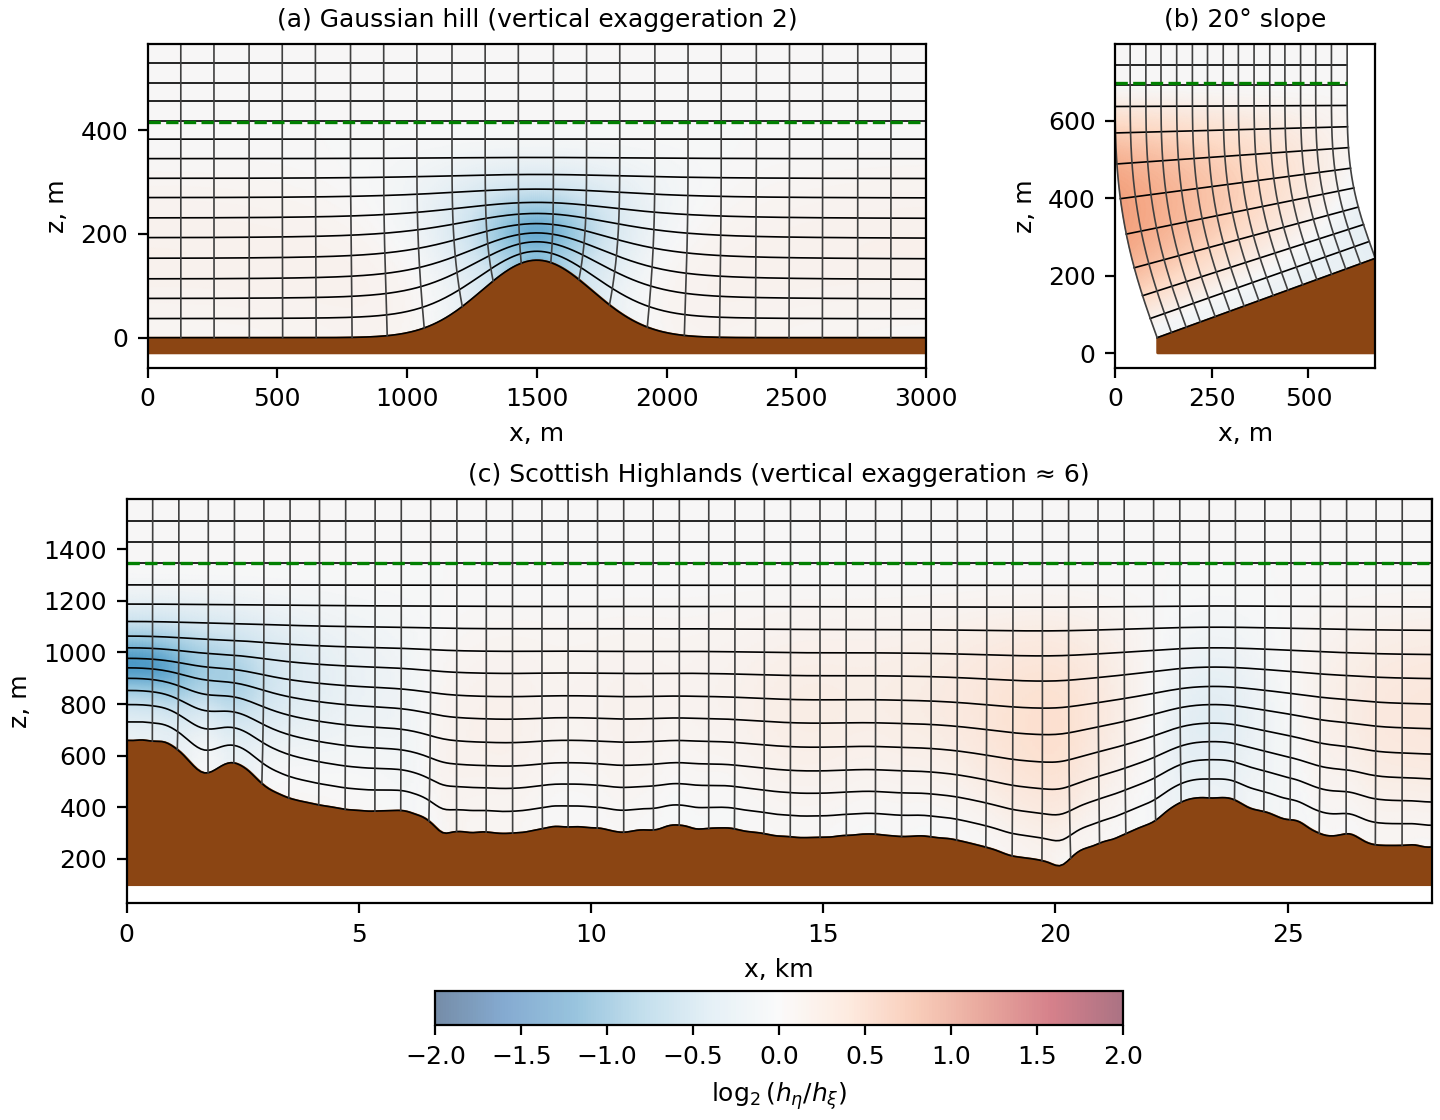
\includegraphics[width=0.85\textwidth]{coordinate_grids_rwp.png}
\caption{Orthogonal terrain-following coordinates. Black: level curves
$\eta=\text{const}$; grey: trajectories $\xi=\text{const}$; color:
$\log_2(h_\eta/h_\xi)$; dashed: top of the transition layer, above which the
coordinates are Cartesian. (a)~Gaussian hill, $z_{\rm ref}=\overline B$,
$L=\SI{400}{m}$. (b)~$20^\circ$ slope without the even extension at $x=0$; the
starting trajectory is then curved. (c)~Scottish Highlands profile of
Section~\ref{sec:highlands}. Panels (a) and (c) are vertically exaggerated, so
the right angles appear distorted.}
\label{fig:grids}
\end{figure*}

%=====================================================================
\section{Transformed One-Way Equation}\label{sec:transformed}

\subsection{Liouville Transformation}
The range dependence of $r$ enters \eqref{eq:helm_orth} through
$\pd_\xi(r\pd_\xi)$. Setting
$\psi=r^{-1/2}\varphi$ and using
$\pd_\xi(r\pd_\xi(r^{-1/2}\varphi))=r^{1/2}\varphi_{\xi\xi}-(r^{1/2})_{\xi\xi}\varphi$,
we obtain
\begin{align}
&\varphi_{\xi\xi}+B\varphi=0,\label{eq:liouville}\\
&B\varphi=r^{-1/2}\pd_\eta\left(\frac{1}{r}\pd_\eta\left(r^{-1/2}\varphi\right)\right)+\left(k^2h_\xi^2-V\right)\varphi,\nonumber
\end{align}
with $V=(r^{1/2})_{\xi\xi}/r^{1/2}$, a term of relative size
$(\lambda/\ell)^2$. The operator $B$ is symmetric in $L^2(d\eta)$.
Dirichlet and Neumann conditions are invariant. Since $\pd_n=h_\eta^{-1}\pd_\eta$
on $\eta=0$, the impedance condition \eqref{eq:leontovich} becomes the Robin
condition
\begin{equation}\label{eq:robin}
\pd_\eta\psi+\gamma\psi=0,\qquad \gamma(\xi)=\alpha\,h_\eta(\xi,0),
\end{equation}
with a coefficient that varies along the ground. The scheme below is written
for $\psi$, so \eqref{eq:robin} is imposed on $\psi$ directly.

\subsection{Flux-Conserving Range Step}
The one-way factorization of \eqref{eq:liouville} retains the transport term,
$\varphi_\xi=i\sqrt B\varphi-\frac14B^{-1}B_\xi\varphi+\dots$, which conserves the
energy flux $\|B^{1/4}\varphi\|^2$ rather than $\|\varphi\|^2$. In the usual PE
for a slowly varying medium this term is neglected. Here it is not negligible:
the coordinate lines rotate with height, so a beam changes its angle to the
local marching direction. The plain step then loses amplitude, by 2--6\% over a
few hundred meters for beams reflected at 40--50$^\circ$ in the tests of
Section~\ref{sec:slope}, in agreement with the WKB factor
$(\cos\theta_1/\cos\theta_2)^{1/2}$. We use the flux-conserving step
\cite{collins1991energy,porter1991energy}. Since the middle factor commutes
with $B_{n+1/2}^{\pm1/4}$, it can be written as
\begin{multline}\label{eq:flux_pairs}
\varphi_{n+1}=\left[B_{n+1}^{-1/4}B_{n+1/2}^{1/4}\right]
e^{i\Delta\xi\sqrt{B_{n+1/2}}}
\left[B_{n+1/2}^{-1/4}B_n^{1/4}\right]\varphi_n\\
=B_{n+1}^{-1/4}e^{i\Delta\xi\sqrt{B_{n+1/2}}}B_n^{1/4}\varphi_n .
\end{multline}
Each bracket is the identity wherever its two columns coincide, in particular
in the whole exterior. The middle factor is approximated by \eqref{eq:rational}
with $L=B/\beta^2-1$.

The factors $(1+L)^{\pm1/4}$ are approximated by rational functions. Their Pad\'e
approximants have poles and zeros on the branch cut $L<-1$, i.e., inside the
evanescent spectrum. There a pair of factors evaluated at slightly different
columns can amplify a spurious mode; we observed a 14\% localized error after
\SI{600}{m}. Following \cite{milinazzo1997}, we take the $[q/q]$ Pad\'e
approximant of $(1+Y)^{1/4}$ with $Y=(1+L)e^{-i\gamma}-1$ and
$\gamma=45^\circ$. Rewritten as factors $(1+cL)/(1+dL)$, its poles and zeros
lie off the real axis. The constant prefactor cancels within each pair, and
only the logarithmic derivative matters, which for $q=2$ is accurate to 5\% up
to $45^\circ$. Since the correction itself is a few percent, the resulting
error is of order $10^{-3}$.

\subsection{Factors in Terms of the Physical Field}
\begin{lemma}\label{lem:psi}
Let $\varphi=r^{1/2}\psi$, $m=r^2$ and
$\het=(k^2h_\xi^2-V)/\beta^2-1$. Then
$r^{3/2}\beta^2(1+cL)\varphi=c\,r\,\pd_\eta(r^{-1}\pd_\eta\psi)+\beta^2m(1+c\het)\psi$.
\end{lemma}
\begin{IEEEproof}
Insert \eqref{eq:liouville} into $\beta^2(1-c)\varphi+cB\varphi$ and multiply by
$r^{3/2}$.
\end{IEEEproof}
Every factor of \eqref{eq:flux_pairs} is therefore the flat scheme
\eqref{eq:substep_flat}, with $\pd_\eta^2$ replaced by the operator
$r\pd_\eta r^{-1}\pd_\eta$ with the variable coefficient $r=h_\eta/h_\xi$, and with
an additional weight $m$. Between columns the field is
rescaled by $(m_{\rm old}/m_{\rm new})^{1/4}$.

%=====================================================================
\section{Discretization}\label{sec:disc}

On the uniform grid $\eta_j=j\Delta\eta$ each factor reads
\begin{multline}\label{eq:scheme}
c\,\delta^2_rv+(1+\alpha\delta^2_r)\left[\tau^2m(1+c\het)v\right]\\
=a\,\delta^2_ru+(1+\alpha\delta^2_r)\left[\tau^2m(1+a\het)u\right]
\end{multline}
with $\tau=\beta\Delta\eta$ and
$\delta^2_r u_j=r_j\left[(u_{j+1}-u_j)/r_{j+1/2}-(u_j-u_{j-1})/r_{j-1/2}\right]$.
For $g=\ln r$ and $D=r\pd r^{-1}\pd$, a Taylor
expansion gives
$\delta^2_r/\Delta\eta^2=D+\frac{\Delta\eta^2}{12}D^2+\Delta\eta^2E+O(\Delta\eta^4)$,
where $E\psi=\frac{1}{24}\left[(g'^2+g'')\psi''+(g'''+g'g''-g'^3)\psi'\right]$.
The Numerov weight cancels the $D^2$ term. The scheme is thus fourth-order in
the wave part, with a second-order error of relative size
$(\Delta\eta/\ell_\eta)^2/24$, negligible since $\ell_\eta\gtrsim L$.

At the ground the Dirichlet unknown is eliminated from the system rather than
imposed by a unit row; a unit row next to entries of order $\alpha\tau^2$ is
satisfied by a pivoting solver only up to amplified round-off. The Neumann
condition uses a mirror node. The impedance closure is described in
Section~\ref{sec:impedance}. The coefficients $\het$, $m$, $r$ are tabulated
on coarse columns, only below the Cartesian region, and are interpolated
linearly in range; the main chain is evaluated at the midpoint. One step
(Algorithm~1) costs $p+4q$ tridiagonal solves, and the $4q$ flux
solves are restricted to the transition layer.

\begin{figure}[!t]
\renewcommand{\algorithmicrequire}{\textbf{Input:}}
\hrule\vspace{2pt}
\textbf{Algorithm 1:} one range step
\vspace{2pt}\hrule
\begin{algorithmic}[1]
\STATE interpolate $(\het,m,r)$ at $\xi_n$, $\xi_{n+1/2}$, $\xi_{n+1}$
\STATE $\psi\leftarrow C_1\psi$ (first bracket of \eqref{eq:flux_pairs}; rows below $\etal$ plus a margin)
\FOR{$l=1,\dots,p$}
\STATE solve \eqref{eq:scheme} with $(a_l,b_l)$ at $\xi_{n+1/2}$ and the NLBC row \eqref{eq:nlbc}
\ENDFOR
\STATE $\psi\leftarrow C_2\psi$ (second bracket of \eqref{eq:flux_pairs})
\end{algorithmic}
\hrule
\end{figure}

\subsection{Impedance Ground}\label{sec:impedance}
For the Robin condition \eqref{eq:robin} a ghost node $u_{-1}$ is added to the
row $j=0$ of \eqref{eq:scheme}, and the system is closed by
\begin{equation}\label{eq:closure}
\left(u_1-u_{-1}\right)+\frac{g}{3}\left(u_{-1}+4u_0+u_1\right)=0,\qquad g=\gamma\Delta\eta .
\end{equation}
This is \eqref{eq:robin} written with the compact (Pad\'e) pair
$(u_1-u_{-1})/(2\Delta\eta)=\psi'_0+\frac{\Delta\eta^2}{6}\psi'''_0+\dots$ and
$(u_{-1}+4u_0+u_1)/6=\psi_0+\frac{\Delta\eta^2}{6}\psi''_0+\dots$
\cite{lele1992compact}. The $\Delta\eta^2$ terms combine into
$\pd_\eta^2(\psi'+\gamma\psi)$. For frozen coefficients the equation turns
$\pd_\eta^2$ into an operator along the ground, which annihilates
\eqref{eq:robin}, so the closure is fourth-order accurate. Relation \eqref{eq:closure} expresses
$u_{-1}$ through $u_0$ and $u_1$, so the system stays tridiagonal. The
coefficients of row $0$ at the ghost node are extrapolated quadratically, and the
same closure is used in all $p+4q$ factors of a step. The usual closure is
the central difference $(u_1-u_{-1})/(2\Delta\eta)+\gamma u_0=0$, as in the
discrete mixed Fourier transform of split-step solvers \cite{dockery1996dmft}.
We call it the mirror closure; it is second-order accurate.

%=====================================================================
\section{Discrete Dispersion Analysis}\label{sec:dispersion}

Freeze $h_\xi$, $h_\eta$ and $k$, and consider a plane wave at angle
$\theta$ to the local marching direction: $k_z=k\sin\theta$, computational
wavenumber $q=k_zh_\eta$, $\psi^n_j=\lambda^ne^{iqj\Delta\eta}$. The flux
factors cancel. With $s=\sin^2(q\Delta\eta/2)$, the symbol of \eqref{eq:scheme}
is
\begin{equation}\label{eq:Lh}
L_h(q)=\het-\frac{4}{\tau^2r^2}\,\frac{s}{1-4\alpha s},\qquad\lambda=R\left(L_h(q)\right),
\end{equation}
and the exact factor is $e^{i\Delta\xi(p-\beta)}$ with $p=h_\xi k\cos\theta$.
The dispersion error per unit physical length is
\begin{equation}\label{eq:disp}
\varepsilon(\theta)=\frac{\left|\log\left(\lambda e^{-i\Delta\xi(p-\beta)}\right)\right|}{h_\xi\Delta\xi}.
\end{equation}

\begin{theorem}[Local equivalence]\label{thm:equiv}
$\varepsilon(\theta;\beta,\Delta\xi,\Delta\eta,h_\xi,h_\eta)=\varepsilon_0(\theta;\beta/h_\xi,h_\xi\Delta\xi,h_\eta\Delta\eta)$,
where $\varepsilon_0$ is the dispersion error of the flat scheme
\eqref{eq:substep_flat} with the given reference wavenumber and steps.
\end{theorem}
\begin{IEEEproof}
Let $\beta_e=\beta/h_\xi$, $\Delta x_e=h_\xi\Delta\xi$ and
$\Delta z_e=h_\eta\Delta\eta$. Then:
\begin{itemize}
\item $\beta\Delta\xi=\beta_e\Delta x_e$, and the coefficients of $R$ depend on
this product only;
\item $\het=k^2/\beta_e^2-1$;
\item $\tau r=\beta_e\Delta z_e$;
\item $q\Delta\eta=k_z\Delta z_e$.
\end{itemize}
Hence $L_h$ and $\lambda$ coincide, and
$e^{i\Delta\xi(h_\xi k\cos\theta-\beta)}=e^{i\Delta x_e(k\cos\theta-\beta_e)}$.
\end{IEEEproof}

\begin{figure}[!t]\centering
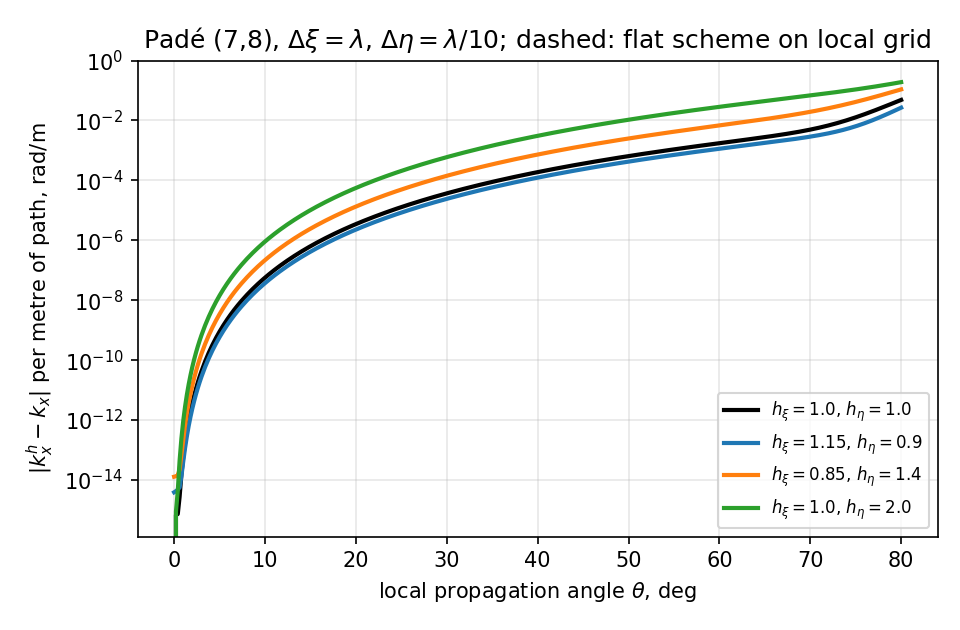
\includegraphics[width=\columnwidth]{disp_local_equivalence.png}\\[1mm]
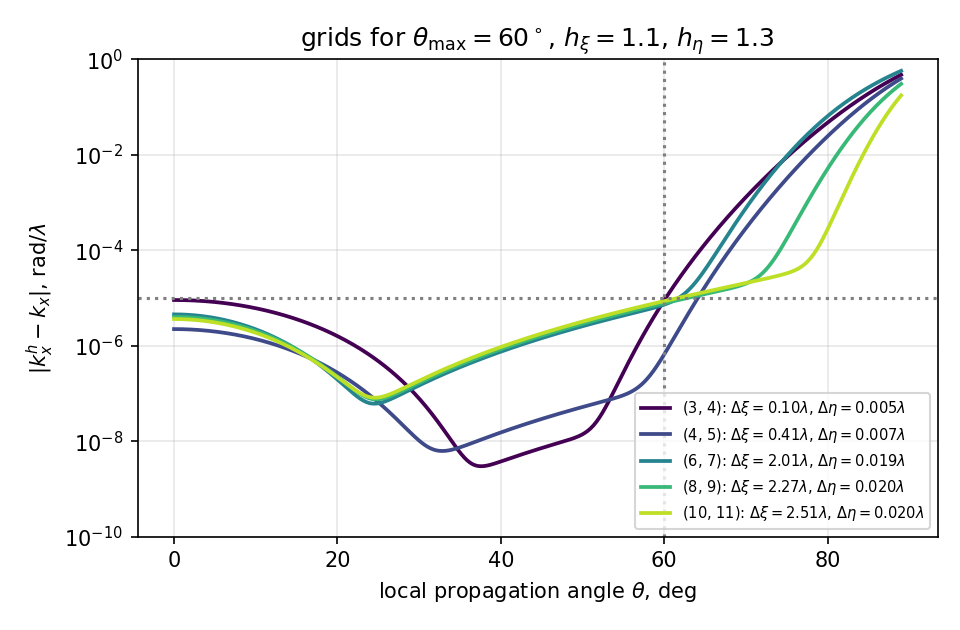
\includegraphics[width=\columnwidth]{disp_orders.png}
\caption{Top: dispersion error for several metric values on one grid (solid)
and of the flat scheme on the local effective grid (dashed); they agree to
$4\cdot10^{-13}$ of the maximum error (Theorem~\ref{thm:equiv}). Bottom:
Pad\'e orders $(3,4)$--$(10,11)$ on grids selected for a $60^\circ$ aperture in a
distorted cell ($h_\xi=1.1$, $h_\eta=1.3$).}
\label{fig:dispersion}
\end{figure}

\begin{corollary}[Angles]
The transformation introduces no angle restriction. A wave is resolved if its
angle to the local marching direction lies within the aperture of the rational
approximation on the local grid. Waves reflected by slopes of up to $\theta_s$
reach $\theta_{\max}+2\theta_s$, so the aperture is set to that value. This
requirement is physical and applies equally to a staircase.
\end{corollary}

\begin{corollary}[Grid selection]
Let $h_\pm=\max/\min h_\xi$. The flat-terrain optimizer
\cite{lytaev2020iccsa,lytaev2026nmp} is applied with:
\begin{itemize}
\item the wavenumber interval $[k_{\min}h_-,k_{\max}h_+]$;
\item the vertical wavenumber bound $k_z^{\max}h_-$;
\item the error budget per unit computational length.
\end{itemize}
The vertical step it returns is divided by $\max r\cdot h_+/h_-$.
\end{corollary}

Fig.~\ref{fig:dispersion} confirms Theorem~\ref{thm:equiv} numerically. It also
shows that every Pad\'e order reaches the target accuracy up to the aperture in
transformed coordinates.

\subsection{Discrete Reflection by the Impedance Ground}
The same frozen-coefficient analysis applies to the ground closure.

\begin{proposition}\label{prop:refl}
Let a discrete wave $u_j=e^{-iqj}+R_he^{iqj}$, $q=k\sin\phi\,h_\eta\Delta\eta$,
satisfy the interior rows of \eqref{eq:scheme}. Then the closure
\eqref{eq:closure} gives
\begin{equation}\label{eq:Rh}
R_h=\frac{iS(q)-g}{iS(q)+g},\qquad S(q)=\frac{3\sin q}{2+\cos q}=q-\frac{q^5}{180}+O(q^7),
\end{equation}
whereas the exact coefficient is $R=(iq-g)/(iq+g)$. The mirror closure gives
\eqref{eq:Rh} with $S=\sin q=q-q^3/6+\dots$. If $\operatorname{Re}\Delta_g\ge0$,
then for both closures, with $\sigma=S(q)/q$,
\begin{equation}\label{eq:Rbound}
|R_h-R|\le\frac{2|1-\sigma|}{\sigma}\approx\begin{cases}q^4/90, & \text{compact},\\ q^2/3, & \text{mirror},\end{cases}
\end{equation}
uniformly in the ground parameters.
\end{proposition}
\begin{IEEEproof}
Since the wave satisfies the interior rows, row $0$ holds iff the ghost value
$e^{iq}+R_he^{-iq}$ satisfies \eqref{eq:closure}, i.e.
$2i\sin q\,(R_h-1)+\frac{g}{3}(4+2\cos q)(1+R_h)=0$, which is \eqref{eq:Rh}. Let
$w=g/(iq)=\Delta_g/\sin\phi$. Then $R=(1-w)/(1+w)$, $R_h=(\sigma-w)/(\sigma+w)$
and $R_h-R=2w(\sigma-1)/[(\sigma+w)(1+w)]$. For $\operatorname{Re}w\ge0$ we have
$|w|\le|1+w|$ and $|\sigma+w|\ge\sigma$.
\end{IEEEproof}

The condition $\operatorname{Re}\Delta_g\ge0$ holds for any passive ground with
$\operatorname{Re}\varepsilon\ge0$, for both polarizations. The bound depends
only on the vertical wavenumber resolved by the grid, as the interior
dispersion error does. A grid that resolves a wave in the interior therefore
also reflects it accurately, whatever the ground. Fig.~\ref{fig:refl} shows
$|R_h-R|$ for wet ground. At $k\Delta\eta=0.5$ the compact closure
is accurate to $6\cdot10^{-5}$ up to $60^\circ$, and the mirror closure to
$10^{-2}$.

\begin{figure}[!t]
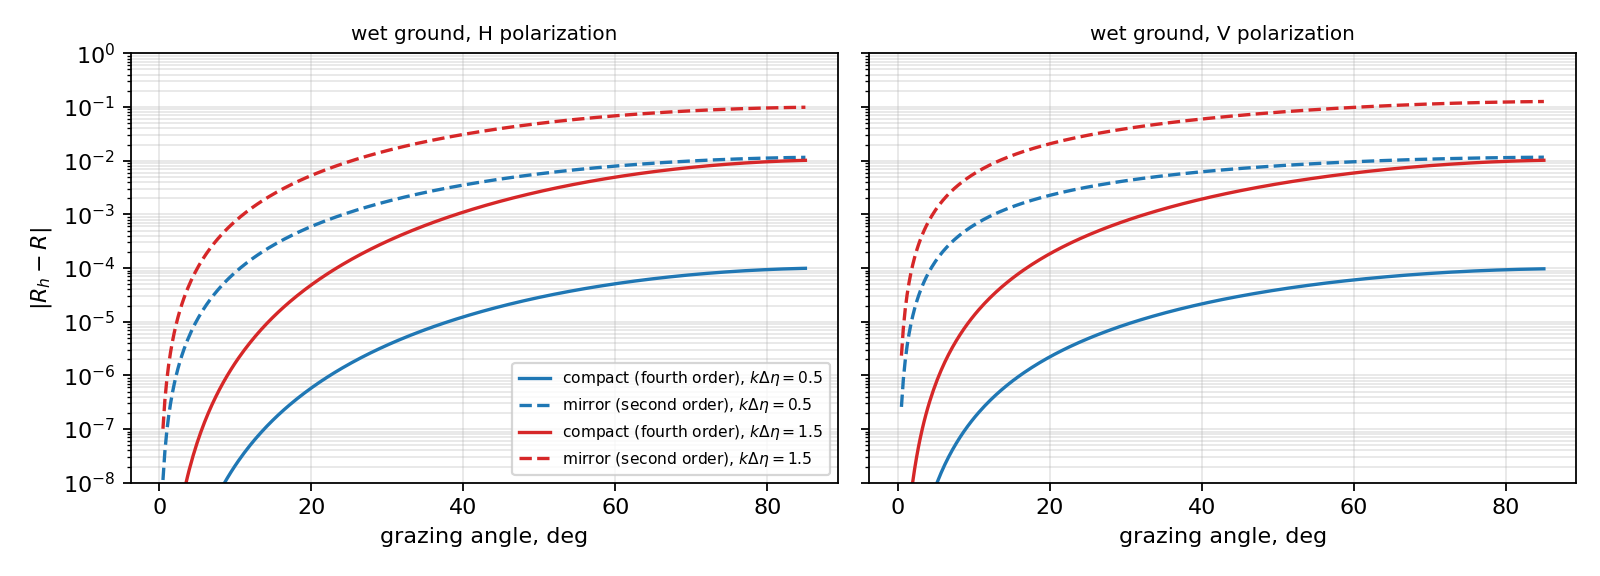
\includegraphics[width=\columnwidth]{impedance_refl_error.png}
\caption{Error of the discrete reflection coefficient of the impedance ground
($\varepsilon=25+1.2i$, \SI{300}{MHz}) for the compact closure
\eqref{eq:closure} (solid) and the mirror closure (dashed), $h_\eta=1$.}
\label{fig:refl}
\end{figure}

%=====================================================================
\section{Compatibility With the Nonlocal Boundary Condition}\label{sec:nlbc}

\begin{theorem}\label{thm:nlbc}
Let $\eta_{\max}\ge\etal+2\Delta\eta$, and let the medium above the transition
layer be range-independent. Then the NLBC \eqref{eq:nlbc} computed for the
chain $R$ and the untransformed exterior scheme is the exact discrete
transparent boundary condition of the scheme of Algorithm~1.
\end{theorem}
\begin{IEEEproof}
For $j\Delta\eta\ge\etal$ we have $h_\xi=h_\eta=r=m=1$ and $V=0$
exactly, because the taper is $C^2$. The rows there coincide with
\eqref{eq:substep_flat} with $z=\eta+z_{\rm ref}$. The flux pairs are the
identity in this region, and are solved below it with the top value passed
through. What reaches the boundary is therefore produced by the chain $R$
alone, with exterior coefficients independent of $n$, and the derivation of
\cite{lytaev2018awpl} applies verbatim, including a linear (Airy) exterior
profile.
\end{IEEEproof}

\begin{remark}
Placing the flux factors around $R$ as in the second line of
\eqref{eq:flux_pairs} is also correct, but the NLBC would then have to be
computed for a chain of $p+2q$ factors containing reciprocal pairs. The matrix
function of the inverse $z$-transform becomes defective, and the adaptive
quadrature of the kernels does not converge. The bracketed form avoids this,
and the kernels are the same as over flat ground.
\end{remark}

%=====================================================================
\section{Comparison With Shift-Map Finite-Difference PEs}\label{sec:shiftmap}

\subsection{The Shift-Map Schemes as Rational Propagators}
With $\zeta=z-T(x)$ and the gauge
\begin{equation}\label{eq:gauge}
u=v\exp\left(ik_0T'\zeta+\tfrac{ik_0}{2}\textstyle\int_0^xT'^2dx'\right),
\end{equation}
the NA PE over the terrain $T$ becomes the NA PE over flat ground for $v$, with
the index $n^2-2\zeta T''$ \cite{beilis1979coupled,barrios1994tpem}. The WA
shift-map PEs apply the same transformation and replace the NA operator by a WA
one \cite{donohue2000gtpe,holm2007wasm}. In the FD schemes surveyed in the
introduction, the envelope satisfies $u_x=ik_0(f(X)-1)u$ with
$X=k_0^{-2}\pd^2_\zeta+n^2-1$, where $f$ approximates $\sqrt{1+X}$ by one of:
\begin{itemize}
\item NA: $f=1+X/2$;
\item Claerbout: $f=(1+\frac34X)/(1+\frac14X)$;
\item Greene: $f=(0.99987+0.79624X)/(1+0.30102X)$;
\item Pad\'e $[2/2]$: $f=(1+\frac54X+\frac5{16}X^2)/(1+\frac34X+\frac1{16}X^2)$.
\end{itemize}
The range step is Crank--Nicolson,
\begin{equation}\label{eq:cn}
u^{n+1}=\frac{1+i\kappa(f(X)-1)}{1-i\kappa(f(X)-1)}\,u^n,\qquad\kappa=\frac{k_0\Delta x}{2}.
\end{equation}
$X$ is discretized by three-point (second-order) or five-point (fourth-order)
differences.

In this form the schemes are rational functions of the vertical operator, of
degree $(1,1)$ or $(2,2)$, exactly like \eqref{eq:rational}. The difference lies
in what is approximated. Equation \eqref{eq:cn} first approximates the square
root and then the exponential by the second-order Cayley transform, so its
error grows with $k_0\Delta x$ and with the angle independently of the order of
$f$. Equation \eqref{eq:rational} approximates the propagator
$e^{i\beta\Delta x(\sqrt{1+L}-1)}$ itself, to order $2p$ in $L$. Its error
vanishes uniformly as the order increases, for range steps of many wavelengths.
The baseline solvers used below implement \eqref{eq:gauge}--\eqref{eq:cn} in the
same code as the proposed method, with the Numerov weight $\alpha$ set to zero.
The two families therefore differ only in the approximation.

\subsection{Grid-Independent Error of the Shift Map}
For a constant slope $s=\tan\theta_s$, substituting a plane wave into the
gauge \eqref{eq:gauge} gives the error of the shift-map PE in the limit
$\Delta x,\Delta\zeta\to0$. A plane wave at the angle $\alpha$ to the horizontal
has $v\propto e^{ik_0(\sin\alpha-s)\zeta}$. The PE propagates it with the
longitudinal wavenumber $k_0[f(-(\sin\alpha-s)^2)-1]$, whereas the exact
wavenumber is $k_0(\cos\alpha+s\sin\alpha-1-s^2/2)$. Hence
\begin{equation}\label{eq:floor}
\varepsilon_\infty(\alpha;\theta_s)=k_0\left|f\left(-(\sin\alpha-s)^2\right)+\frac{s^2}{2}-s\sin\alpha-\cos\alpha\right|,
\end{equation}
after removal of the angle-independent part $f(0)-1$. For $f=1+X/2$ this is
$k_0|1-\frac12\sin^2\alpha-\cos\alpha|$, independent of the slope: the BT
transformation is exact for the NA PE, and its floor is that of the NA PE on
flat ground. For any other $f$, including the exact square root, the floor
depends on the slope. It vanishes only on a narrow set of angles because the
gauge is paraxial.

Fig.~\ref{fig:floor} shows \eqref{eq:floor} as a function of the angle to the
slope. At an accuracy of $10^{-4}$\,rad$/\lambda$ (\SI{0.1}{rad} over
$10^3\lambda$), the admissible angles are as follows.
\begin{itemize}
\item \emph{Exact square root (any WA scheme):} only waves between $3.9^\circ$
and $6.3^\circ$ above the horizontal on a $10^\circ$ slope, a single angle on a
$20^\circ$ slope, and none on a $30^\circ$ slope.
\item \emph{Claerbout approximation:} the same windows on slopes. On these
slopes the floor is set by the gauge, not by the square-root approximation, so
raising the order of $f$ cannot help.
\item \emph{NA PE:} $|\alpha|<5.9^\circ$ for every slope.
\end{itemize}
This quantifies the published observations: WA shift maps are limited to slopes
of 10--20$^\circ$, can be worse than the NA PE on lee-side slopes
\cite{wang2020smpe,zhou2017lfhighangle}, and their sheared vertical wavenumber
is unphysical \cite{gilbert2022wabt}. In the proposed coordinates, by
Theorem~\ref{thm:equiv}, the frozen-coefficient error is that of the flat
scheme on a local grid, and it vanishes under refinement for every slope.

\begin{figure*}[!t]\centering
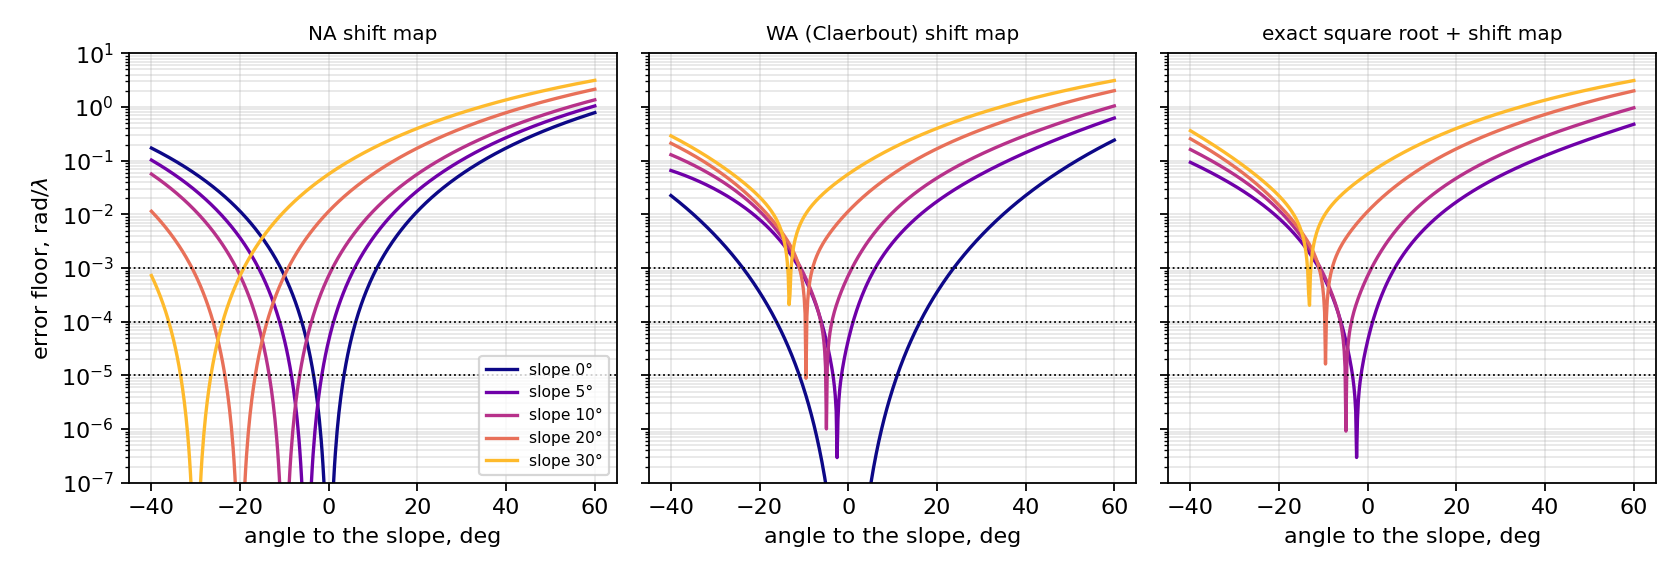
\includegraphics[width=0.92\textwidth]{shiftmap_slope_floor.png}
\caption{Grid-independent error \eqref{eq:floor} of the shift map on a slope,
versus the angle to the slope, for the NA approximation, the Claerbout
approximation and the exact square root. Dotted: accuracy budgets of $10^{-3}$,
$10^{-4}$ and $10^{-5}$\,rad$/\lambda$. For the proposed coordinates the
corresponding error is zero.}
\label{fig:floor}
\end{figure*}

\subsection{Maximum Angle and Cost on Flat Ground}
On flat ground the shift map plays no role, and the comparison concerns the
propagators alone. For every method, accuracy budget $\varepsilon_{\max}$ and
maximum angle $\theta_{\max}$, we searched by brute force over
$10^{-2.5}\le\Delta x/\lambda\le10^{2.5}$ and
$10^{-3}\le\Delta z/\lambda\le1$, and over
$\beta\in[0.5,1]k_0$ for the rational scheme. The cheapest grid is the one for
which the dispersion error \eqref{eq:disp}, with the same Numerov or FD symbols,
stays below $\varepsilon_{\max}$ for all $\theta\le\theta_{\max}$. The cost is
the number of tridiagonal solves per $\lambda^2$, $p/(\Delta x\Delta z)$. The
pentadiagonal systems of the five-point schemes are counted as one solve, which
favors the FD methods. A phase drift common to all angles (Greene: $f(0)\ne1$;
rational: $\beta\ne k_0$) is a global phase and is removed for all methods.

\begin{table}[!t]\centering
\caption{Maximum Propagation Angle (Degrees) Meeting an Accuracy Budget}\label{tab:maxangle}
\setlength{\tabcolsep}{4pt}
\begin{tabular}{lccc}\toprule
budget, rad$/\lambda$ & $10^{-3}$ & $10^{-4}$ & $10^{-5}$\\
(0.1 rad over) & ($10^2\lambda$) & ($10^3\lambda$) & ($10^4\lambda$)\\\midrule
NA-FD, CN, 3-point & 10.8 & 6.0 & 3.3\\
WA-FD Claerbout, CN, 3-point & 23.8 & 16.0 & 11.0\\
WA-FD Greene, CN, 5-point & 11.8 & 3.3 & 1.0\\
WA-FD Pad\'e $[2/2]$ sqrt, CN, 5-point & 43.8 & 34.8 & 27.8\\\midrule
rational Pad\'e $(1,2)$, Numerov & 43.0 & 38.0 & 27.5\\
rational Pad\'e $(2,3)$, Numerov & 65.3 & 54.5 & 42.8\\
rational Pad\'e $(4,5)$, Numerov & 79.5 & 73.3 & 66.3\\
rational Pad\'e $(6,7)$, Numerov & 82.5 & 80.0 & 78.0\\
rational Pad\'e $(8,9)$, Numerov & 84.3 & 82.3 & 80.5\\
\bottomrule\end{tabular}
\end{table}

\begin{figure}[!t]\centering
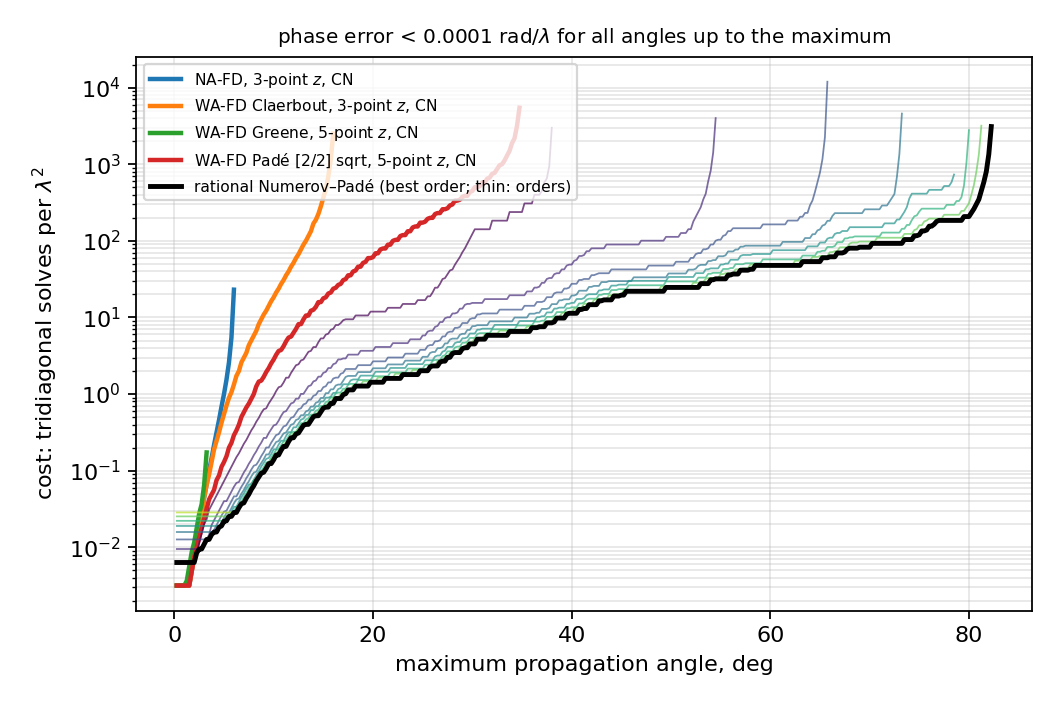
\includegraphics[width=\columnwidth]{shiftmap_efficiency.png}
\caption{Minimal cost (tridiagonal solves per $\lambda^2$) to keep the
dispersion error below $10^{-4}$\,rad$/\lambda$ for all angles up to the
maximum. Thick black: the rational scheme with the best order; thin lines:
individual Pad\'e orders $(1,2)$--$(8,9)$.}
\label{fig:efficiency}
\end{figure}

\begin{figure}[!t]\centering
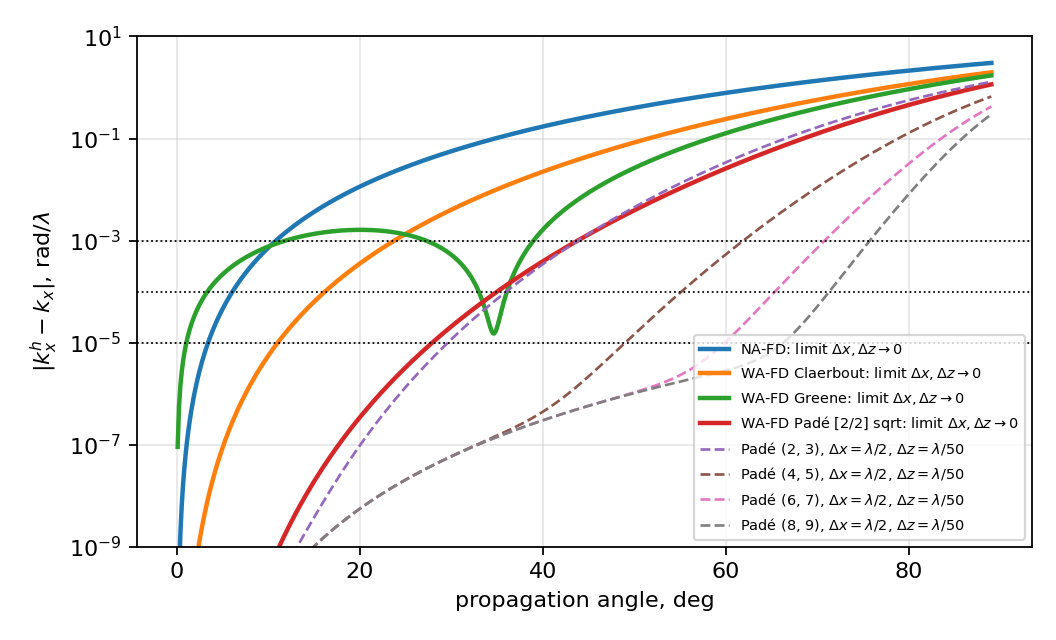
\includegraphics[width=\columnwidth]{shiftmap_error_vs_angle.png}
\caption{Dispersion error versus angle: grid-independent limits of the FD PEs
(solid) and the rational scheme on a coarse grid, $\Delta x=\lambda/2$,
$\Delta z=\lambda/50$ (dashed).}
\label{fig:errangle}
\end{figure}

Table~\ref{tab:maxangle} and Figs.~\ref{fig:efficiency}--\ref{fig:errangle}
show three things.
\begin{itemize}
\item \emph{FD angle limits.} The FD PEs have an angle beyond which no grid
meets the budget, because the error of $f$ does not decrease with the grid
(Fig.~\ref{fig:errangle}). At $10^{-4}$\,rad$/\lambda$ this angle is $6^\circ$
(NA), $16^\circ$ (Claerbout) and $35^\circ$ (Pad\'e $[2/2]$). The Greene
approximation is a minimax fit with a relative error of about $10^{-4}$ over a
wide range of angles; it is useful only for coarser budgets.
\item \emph{No angle limit for the rational scheme.} Its reachable angle grows
with the order without bound, from $38^\circ$ for $(1,2)$ to $82^\circ$ for
$(8,9)$, and reaches $80^\circ$ even at $10^{-5}$\,rad$/\lambda$. The search
interval for $\Delta z$, not the method, ends the curves in
Fig.~\ref{fig:efficiency}.
\item \emph{Cost.} Where both are feasible, the rational scheme is far cheaper.
At $10^{-4}$\,rad$/\lambda$ the cost ratio Claerbout/rational is 130 at
$10^\circ$ and 560 at $15^\circ$, and the ratio Pad\'e-$[2/2]$-FD/rational is
20, 43 and 99 at $10^\circ$, $20^\circ$ and $30^\circ$. The reason is mainly
the range step. The Pad\'e approximation of the propagator is accurate to high
order in $\beta\Delta x$ and allows steps of the order of the wavelength or
more. The Crank--Nicolson step is only second order in $k_0\Delta x(f-1)$, so
its step must shrink quickly as the angle grows.
\end{itemize}

\subsection{Confirmation Against Exact Solutions}
\emph{Beams over flat ground.} Complex-source-point beams (\SI{300}{MHz},
Rayleigh parameter \SI{50}{m}, divergence $2.3^\circ$) were launched at
$5^\circ$--$70^\circ$ over a perfectly conducting ground and propagated over
\SI{300}{m}. NA-FD and WA-FD (Claerbout) were run on a typical grid
($\lambda/2\times\lambda/10$) and on a fine grid ($\lambda/8\times\lambda/40$).
The rational scheme used the grid chosen by its optimizer for the aperture
$\theta+8^\circ$ and precision $10^{-2}$. All three use the NLBC on top, so only
the propagator differs. Fig.~\ref{fig:angles} shows the maximum error with
respect to the exact field.
\begin{itemize}
\item \emph{FD PEs.} WA-FD is accurate at $5^\circ$ but fails at $15^\circ$ (2.6\%
on the fine grid) and beyond. NA-FD exceeds 3\% already at $5^\circ$. Refining
the grid does not help at $30^\circ$ and above, in agreement with
Table~\ref{tab:maxangle}.
\item \emph{Rational scheme.} Its error is $1.6\cdot10^{-3}$ to
$1.4\cdot10^{-4}$ at all angles up to $70^\circ$. At $5^\circ$ it uses 49 times
fewer grid nodes than the typical FD grid, and 790 times fewer than the fine one.
\end{itemize}

\emph{Beam reflected by a slope.} For the exact problem of
Section~\ref{sec:slope} the NA and WA shift maps were run on the fine grid
($\lambda/8\times\lambda/40$). Their maximum errors are 0.67/0.56, 1.02/0.96,
1.41/1.68 and 1.19/1.29 (NA/WA) for slopes of $5^\circ$, $10^\circ$, $20^\circ$
and $30^\circ$. The terrain-following rational solver gives
$8.3\cdot10^{-5}$, $1.4\cdot10^{-4}$, $1.2\cdot10^{-3}$ and $2.9\cdot10^{-3}$.
Already at $5^\circ$ the reflected beam ($20^\circ$) lies outside the
admissible windows of Fig.~\ref{fig:floor}.

\begin{figure}[!t]\centering
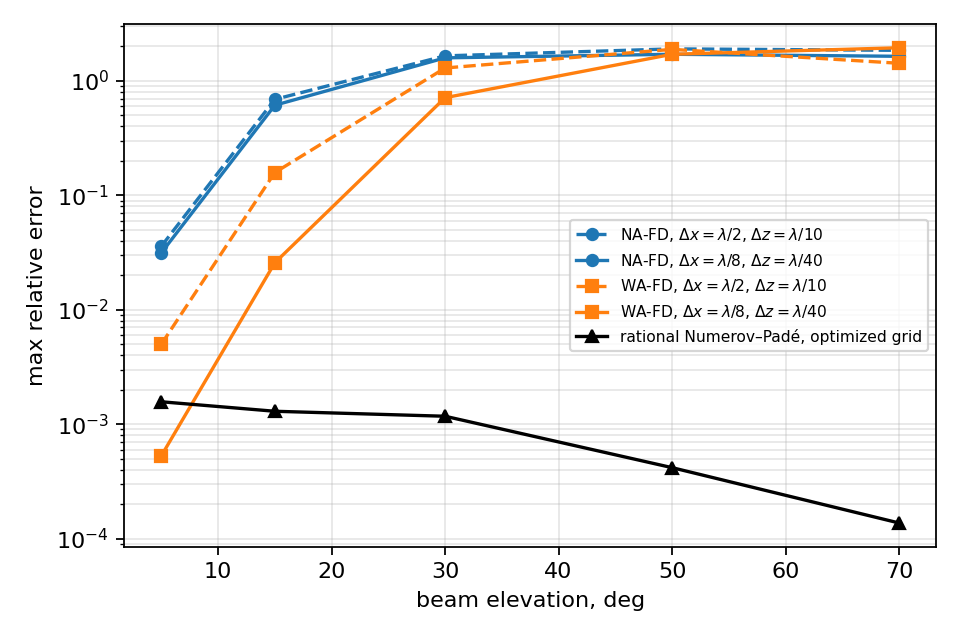
\includegraphics[width=\columnwidth]{shiftmap_comparison_angles.png}
\caption{Beams over flat perfectly conducting ground: maximum error with respect
to the exact solution versus elevation, for NA-FD and WA-FD on two grids and for
the rational scheme on its optimized grid.}
\label{fig:angles}
\end{figure}

%=====================================================================
\section{Discrete NLBC Versus Absorbing Layers}\label{sec:absorber}

Shift-map and split-step PEs truncate the domain by absorbing layers. The
complex-index layer of \cite{khodr2020iterative} is
$n^2\to n^2+iA\left((z-z_a)/D\right)^2$ over a layer of thickness $D$ above the
height of interest $H$, with $\psi=0$ on top; window filters
\cite{zhangp2014window} act similarly. Such a layer works for a range of angles
that depends on $A$ and $D$:
\begin{itemize}
\item a weak or thin layer lets steep waves reach the top and reflect;
\item a strong one reflects grazing waves at its gradient.
\end{itemize}
The discrete NLBC has no parameters: it is exact for the discrete scheme at
every angle.

To isolate the boundary error we used the same propagator in all runs (Pad\'e
$(7,8)$, Numerov, $\Delta x=\SI{2.5}{m}$, $\Delta z=\SI{0.1}{m}$ at
\SI{300}{MHz}), and only the top boundary was changed. On this grid the
propagation error is small. With the NLBC, a domain \SI{200}{m} taller gives the
same field to all digits. The setup is:
\begin{itemize}
\item beams at $1^\circ$, $3^\circ$, $10^\circ$ and $30^\circ$ leave the region
of interest $z<H=\SI{200}{m}$ through the top;
\item the ranges are 17.2, 5.7, 1.7 and \SI{0.5}{km}, so that each beam crosses
$H$ well inside the domain;
\item the NLBC is placed at $H+\SI{20}{m}$;
\item the absorbing layers have $D=H/4$, $H/2$ and $H$, and
$A=10^{-3}$--$1$.
\end{itemize}
Fig.~\ref{fig:absorber} shows the maximum error in $z<H$.

\begin{figure*}[!t]\centering
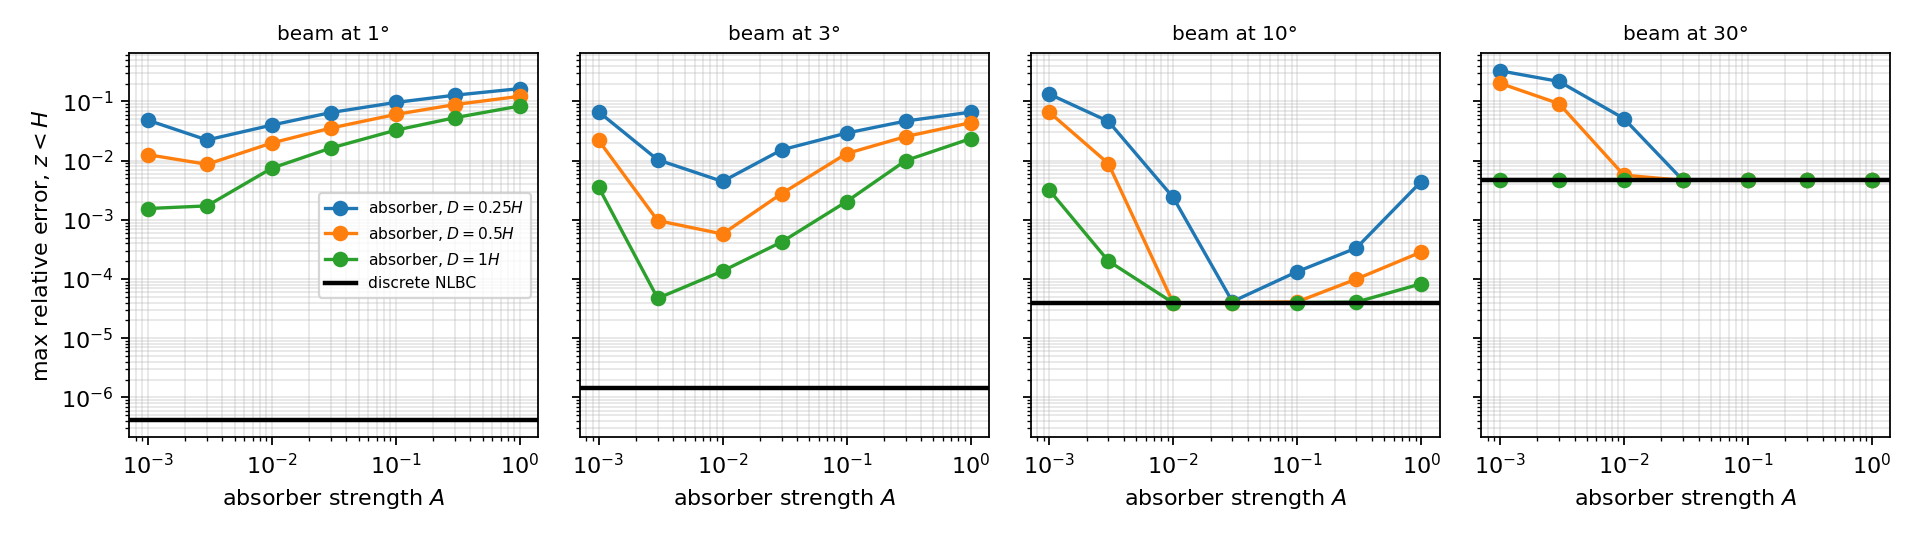
\includegraphics[width=\textwidth]{shiftmap_comparison_absorber.png}
\caption{Maximum error below $H$ for beams leaving the domain through the top:
absorbing layers of thickness $D$ and strength $A$ versus the discrete NLBC
(black). Same propagator and grid in all runs.}
\label{fig:absorber}
\end{figure*}

\begin{itemize}
\item \emph{NLBC accuracy.} With the NLBC the error is $4\cdot10^{-7}$,
$1.4\cdot10^{-6}$ and $4\cdot10^{-5}$ for $1^\circ$, $3^\circ$ and $10^\circ$.
At $30^\circ$ it is $4.6\cdot10^{-3}$, the propagation error of this grid at
that angle, which every boundary shares.
\item \emph{Absorbing layers.} Their errors depend strongly on the angle and on
$(A,D)$. For grazing beams no setting comes close to the NLBC. At $1^\circ$ the
best layer ($D=H$, $A=10^{-3}$) gives $1.6\cdot10^{-3}$, four thousand times the
NLBC error, and stronger layers give up to $8\cdot10^{-2}$. At $3^\circ$ the
best value is $4.7\cdot10^{-5}$ against $1.4\cdot10^{-6}$.
\item \emph{Steep beams.} Weak or thin layers reflect, with errors up to 0.28
for $D=H/4$.
\item \emph{No universal setting.} The value $A=10^{-2}$, $D=H$ is acceptable
from $3^\circ$ upward, but gives $7.5\cdot10^{-3}$ at $1^\circ$. The thinner
layers recommended in the literature ($D\approx0.3H$) are worse.
\end{itemize}
The absorbing layer therefore needs tuning to the angular content of the field,
which is not known in advance. The NLBC needs none.

\emph{Cost.} A layer of thickness $D=H$ doubles the number of vertical nodes;
here, 4001 instead of 2201. The NLBC adds a one-time computation of the
convolution kernels, and at each step a convolution with the history of the
boundary values, $O(p^2N_x)$ operations, independent of the number of vertical
nodes. With the small vertical grids of this test these overheads dominate. The
NLBC runs took 71, 11, 4.3 and \SI{2.8}{s} for $1^\circ$, $3^\circ$,
$10^\circ$ and $30^\circ$ ($N_x=6876$, 2291, 682 and 209). The $D=H$ layers
took 18--22, 5, 1.3 and \SI{0.4}{s}. The relative overhead decreases with the
number of vertical nodes. Recursive or sum-of-exponentials approximations of
the convolution \cite{wangr2017dnlbc3d,arnold_ehrhardt1998jcp} remove its growth
with $N_x$. The gain from the NLBC is therefore reliability and accuracy, not
speed on small grids.

%=====================================================================
\section{Numerical Results}\label{sec:results}

The method is implemented in JAX in the open-source library
\texttt{pywaveprop} \cite{pywaveprop}, as a subclass of its rational propagator.
It reuses the Pad\'e coefficients, the grid optimizer and the NLBC. Over flat
ground it reproduces the existing propagator, including the NLBC, to
$4\cdot10^{-14}$.

\subsection{Exact Solution: Beam Reflected by a Conducting Slope}\label{sec:slope}

The incident field is a \SI{300}{MHz} complex-source-point beam, an exact
solution of the Helmholtz equation. Its waist is at $(-50,30)$\,m, its Rayleigh
parameter is \SI{100}{m}, and it is directed at $-10^\circ$. Its image in the line
$z=x\tan\theta_s$ gives the exact field above the Dirichlet slope; the reflected
beam leaves at $2\theta_s+10^\circ$. Both solvers start from the exact field,
use Pad\'e $(7,8)$ and the aperture $\theta_{\max}=10^\circ+2\theta_s+5^\circ$,
and their grids are chosen by the respective optimizers with precision
$10^{-2}$. Table~\ref{tab:slope} gives the maximum error relative to the
maximum of the exact field, and Fig.~\ref{fig:slope} shows the fields and the
errors.

\begin{table}[!t]\centering
\caption{Exact Slope Test: Relative Maximum Error}\label{tab:slope}
\setlength{\tabcolsep}{3.5pt}
\begin{tabular}{cccccccc}\toprule
& & \multicolumn{3}{c}{terrain-following} & \multicolumn{3}{c}{staircase}\\
\cmidrule(lr){3-5}\cmidrule(lr){6-8}
$\theta_s$ & beam & $\Delta x$, m & $\Delta z$, m & error & $\Delta x$, m & $\Delta z$, m & error\\\midrule
$10^\circ$ & $30^\circ$ & 2.5 & 0.035 & $1.4\cdot10^{-4}$ & 2.5 & 0.063 & 0.54\\
$20^\circ$ & $50^\circ$ & 2.5 & 0.019 & $1.2\cdot10^{-3}$ & 2.5 & 0.035 & 0.69\\
$30^\circ$ & $70^\circ$ & 1.0 & 0.009 & $2.9\cdot10^{-3}$ & 1.0 & 0.016 & 0.81\\
\bottomrule\end{tabular}
\end{table}

\begin{figure*}[!t]\centering
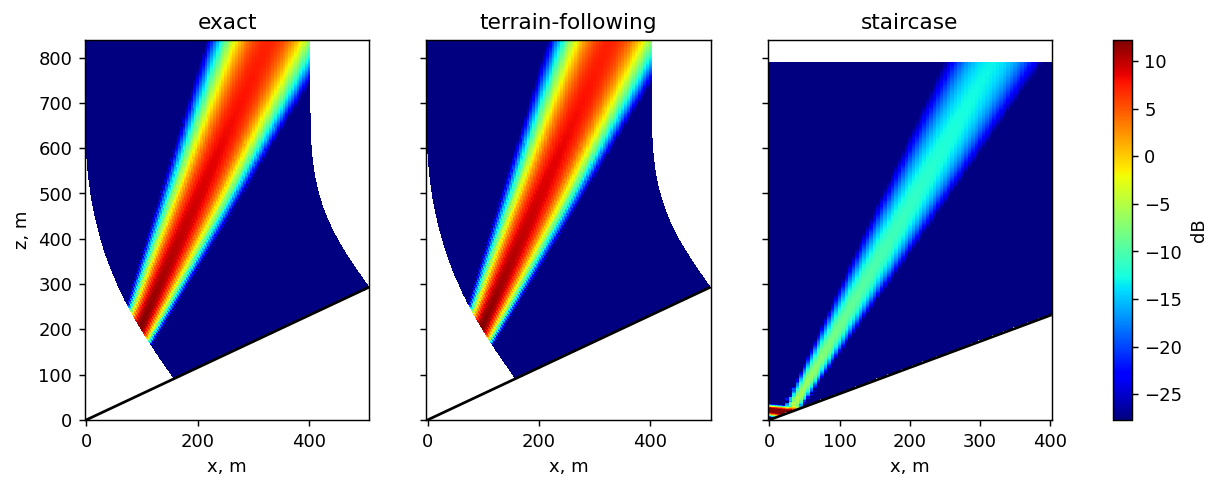
\includegraphics[width=0.78\textwidth]{slope_exact_30deg_maps.png}\\
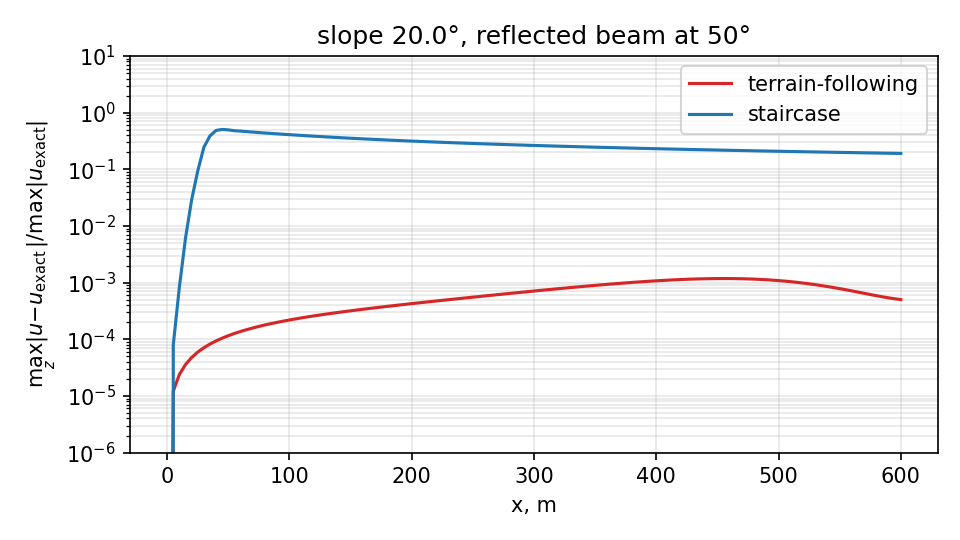
\includegraphics[width=0.42\textwidth]{slope_exact_20deg_error.png}\hspace{4mm}
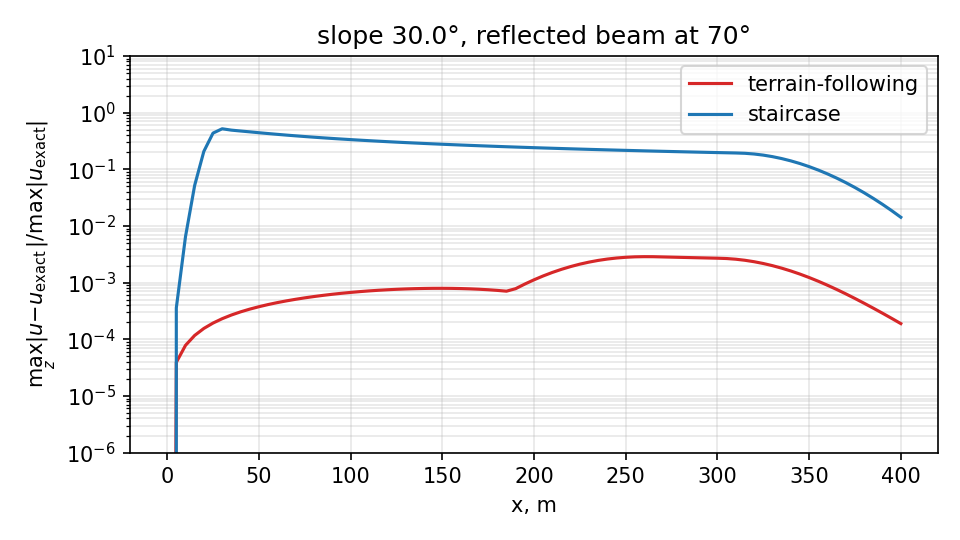
\includegraphics[width=0.42\textwidth]{slope_exact_30deg_error.png}
\caption{Beam reflected by a perfectly conducting slope. Top: $|u|$ for
$\theta_s=30^\circ$ (reflected beam at $70^\circ$); the terrain-following domain
is bounded by the curved trajectories $\xi=0$ and $\xi=x_{\max}$. Bottom: maximum
error over height versus range for $\theta_s=20^\circ$ and $30^\circ$.}
\label{fig:slope}
\end{figure*}

The terrain-following error is $10^{-4}$--$3\cdot10^{-3}$ up to a reflected beam
at $70^\circ$. The staircase loses most of the reflected beam (Fig.~\ref{fig:slope}),
and its error decreases only slowly under refinement. For $\theta_s=20^\circ$
it is 0.69, 0.55 and 0.54 at $\Delta z=0.035$, $0.013$ and \SI{0.005}{m}
($\lambda/200$), and still 0.45 when in addition $\Delta x$ is reduced to
\SI{0.625}{m}. The terrain-following grids have 1.2--1.4 times more vertical
nodes, because of the expansion $\max r$ in the transition layer. Each step
also costs $p+4q$ instead of $p$ solves, so the run time was 7--11 times that
of the staircase, at errors two to three orders of magnitude smaller.

\subsection{Role of the Flux-Conserving Step}

For $\theta_s=20^\circ$, three variants of the range step give:
\begin{itemize}
\item Liouville rescaling alone ($q=0$): error $6.4\cdot10^{-2}$, an amplitude drift
along the reflected beam;
\item unrotated $[2/2]$ flux factors: a spurious evanescent component grows to
0.14;
\item rotated flux factors: $1.2\cdot10^{-3}$.
\end{itemize}
Both ingredients of Section~\ref{sec:transformed} are therefore necessary.

\subsection{Exact Solution: Beam Reflected by an Impedance Slope}\label{sec:impslope}

For the impedance ground the incident beam is written as a superposition of
plane waves with the Gaussian angular spectrum
$\exp[-((\phi-\phi_0)/2^\circ)^2]$, focused at $(-50,30)$\,m and directed at
$-5^\circ$ (waist about \SI{9}{m}). Each plane wave is reflected by the slope with
the coefficient $R(\phi)$ of \eqref{eq:leontovich}, so the sum is an exact
solution of the Helmholtz equation with the impedance condition on the slope. The
spectrum is truncated where it falls below $e^{-36}$; the truncated sum is still
exact. We take three grounds at \SI{300}{MHz}: wet ground ($\varepsilon=25+1.2i$),
dry ground ($4+0.006i$) and sea water ($70+300i$). For V polarization over wet
ground the Brewster angle is $11^\circ$, and the reflected beam is weak and
sensitive to the impedance. The solver uses Pad\'e $(7,8)$, the aperture
$5^\circ+2\theta_s+8^\circ$, and the grid of its optimizer for precision
$10^{-2}$. Table~\ref{tab:impslope} gives the error over the whole domain.

\begin{table}[!t]\centering
\caption{Exact Impedance-Slope Test: Relative Maximum Error}\label{tab:impslope}
\setlength{\tabcolsep}{4pt}
\begin{tabular}{cccccc}\toprule
$\theta_s$ & ground & $\Delta x$, m & $\Delta\eta$, m & H & V\\\midrule
$5^\circ$ & wet & 2.5 & 0.063 & $4.4\cdot10^{-5}$ & $3.9\cdot10^{-5}$\\
$10^\circ$ & wet & 2.5 & 0.037 & $9.2\cdot10^{-5}$ & $3.0\cdot10^{-5}$\\
$10^\circ$ & dry & 2.5 & 0.037 & $8.2\cdot10^{-5}$ & $3.8\cdot10^{-5}$\\
$10^\circ$ & sea & 2.5 & 0.037 & $9.6\cdot10^{-5}$ & $8.1\cdot10^{-5}$\\
$20^\circ$ & wet & 2.5 & 0.020 & $8.1\cdot10^{-4}$ & $8.2\cdot10^{-4}$\\
$30^\circ$ & wet & 1.25 & 0.010 & $9.3\cdot10^{-4}$ & $9.2\cdot10^{-4}$\\
\bottomrule\end{tabular}
\end{table}

The error is below $10^{-3}$ for all grounds and both polarizations, up to a
reflected beam at $65^\circ$, and is of the same size as for the conducting
slope. To isolate the ground closure, the case $\theta_s=10^\circ$ over wet
ground was repeated on prescribed grids ($\Delta x=\SI{2.5}{m}$,
$\beta=k\cos20^\circ$) with both closures:

\begin{center}
\setlength{\tabcolsep}{4pt}
\begin{tabular}{ccccc}\toprule
$k\Delta\eta$ & 0.39 & 0.63 & 1.05 & 1.57\\\midrule
V, compact & $7.5\cdot10^{-5}$ & $2.5\cdot10^{-4}$ & $1.7\cdot10^{-3}$ & $8.6\cdot10^{-3}$\\
V, mirror  & $7.6\cdot10^{-4}$ & $1.9\cdot10^{-3}$ & $5.4\cdot10^{-3}$ & $1.3\cdot10^{-2}$\\
H, both    & $2.6\cdot10^{-4}$ & $8.1\cdot10^{-4}$ & $5.4\cdot10^{-3}$ & $2.7\cdot10^{-2}$\\
\bottomrule\end{tabular}
\end{center}

For V polarization the mirror closure dominates the error on fine grids, and the
compact closure reduces it by a factor of 3--10. For H polarization
$|w|=|\Delta_g|/\sin\phi\approx20$, so $|R_h-R|\approx2|1-\sigma|/|w|$ is small
for both closures, and the error is that of the interior scheme. The compact
closure costs nothing extra, since the system remains tridiagonal.

\subsection{Real Terrain and NWP Refractivity}\label{sec:highlands}

A \SI{300}{MHz} horizontally polarized antenna on a \SI{30}{m} mast stands on
top of a ridge in the Scottish Highlands (\ang{57.2163}N \ang{4.9214}W) and
radiates along a \SI{28}{km} path to \ang{57.40}N \ang{4.60}W. Its beam is
$4^\circ$ wide and tilted $1^\circ$ down.
\begin{itemize}
\item \emph{Terrain:} SRTM-type elevation at \ang{0.0005}, from 166 to \SI{664}{m},
smoothed with $\sigma=\SI{100}{m}$; the maximum slope is $11.1^\circ$.
\item \emph{Refractivity:} the modified refractivity of the GFS analysis of
2026-10-09 12~UTC, interpolated along the path and averaged over range.
\item \emph{Ground:} perfectly conducting.
\item \emph{Grid parameters:} aperture $5^\circ+2\cdot11.1^\circ$, transition
height $L=\SI{1000}{m}$, $z_{\rm ref}=\overline B$.
\end{itemize}
Both solvers see the same smoothed terrain. Fig.~\ref{fig:highlands} shows the
path loss.

\begin{figure*}[!t]\centering
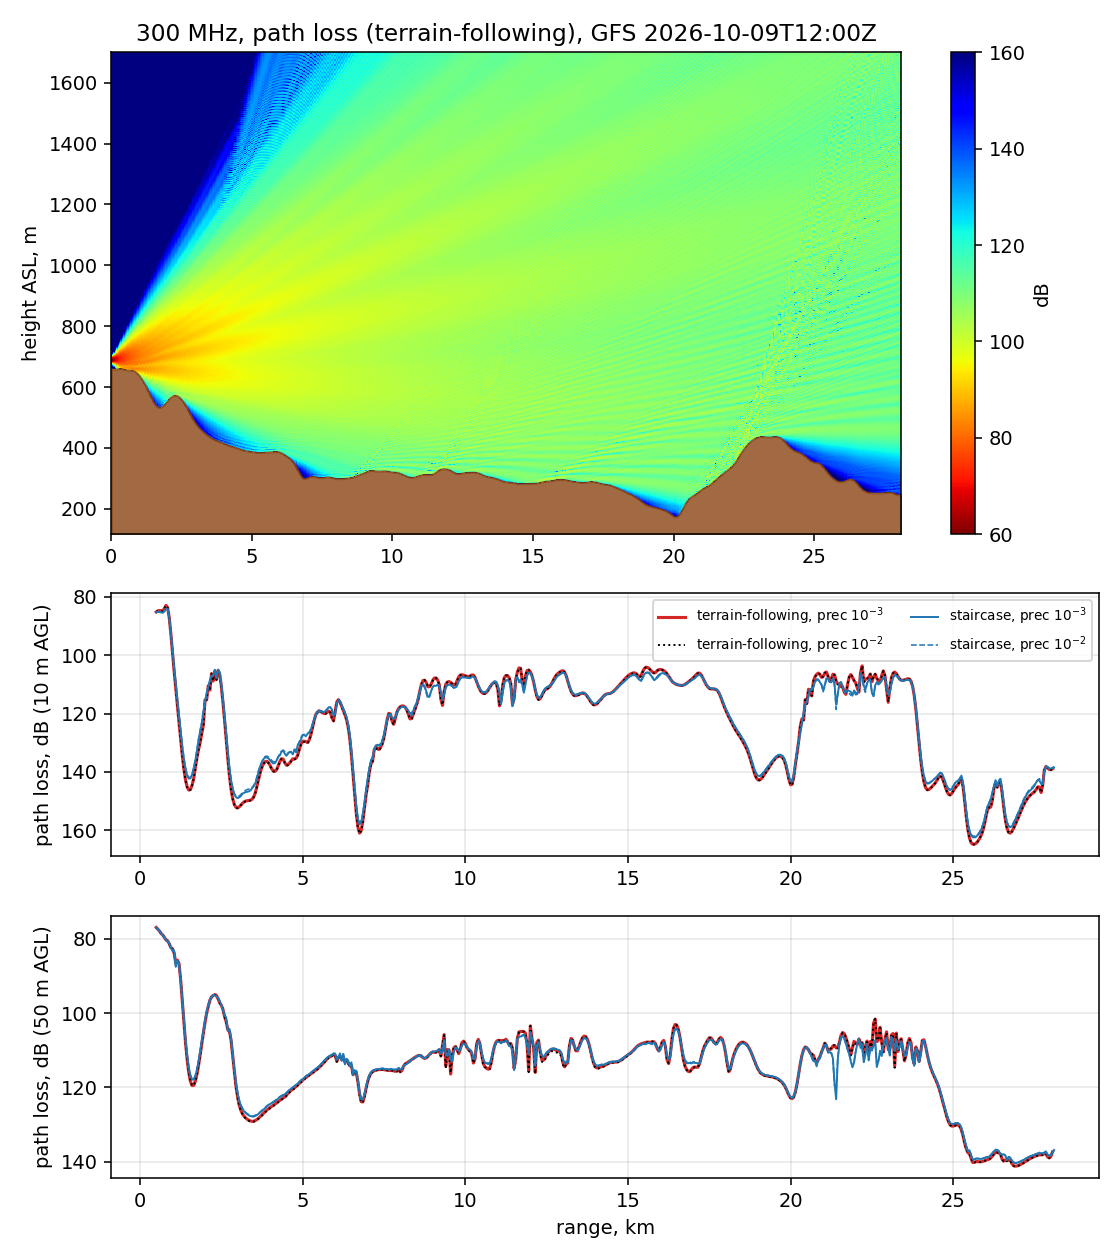
\includegraphics[width=0.62\textwidth]{troposphere_highlands.png}\hspace{2mm}
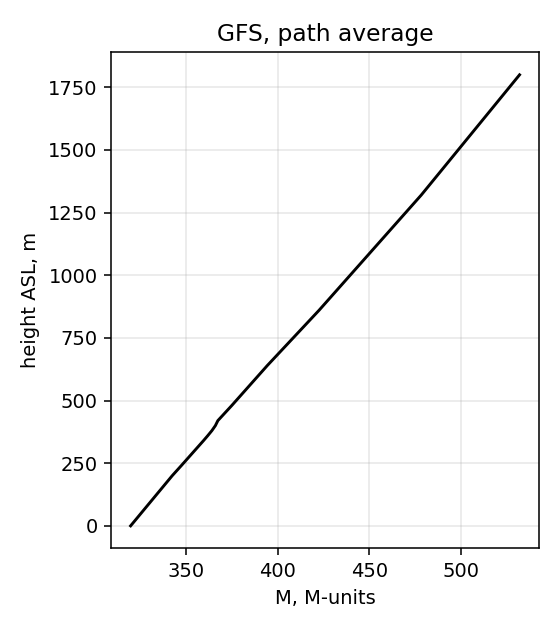
\includegraphics[width=0.22\textwidth]{troposphere_highlands_M.png}
\caption{Scottish Highlands, \SI{300}{MHz}. Left: path loss of the
terrain-following solver, and path loss \SI{10}{m} and \SI{50}{m} above the
ground for both solvers at two precision settings. Right: GFS modified
refractivity averaged along the path.}
\label{fig:highlands}
\end{figure*}

Each solver is converged with respect to its own grid. The two precision
settings ($10^{-2}$ and $10^{-3}$) differ, at \SI{10}{m} above the ground, by
\SI{0.08}{dB} (median) for the terrain-following solver and by \SI{0.15}{dB} for
the staircase. The two solvers differ by \SI{1.1}{dB} at \SI{10}{m} and
\SI{0.44}{dB} at \SI{50}{m} above the ground. The largest differences, up to a
few decibels, occur on the slopes facing the transmitter, where the staircase
solution carries small-scale ripple consistent with scattering by the steps
(Section~\ref{sec:slope}). The terrain-following runs took 468 and \SI{1390}{s}
on a CPU, against 73 and \SI{117}{s} for the staircase. The terrain-following
grid ($\Delta x=\SI{3.1}{m}$, $\Delta\eta=0.034$ and \SI{0.019}{m}) is finer
because of the metric spread $h_\xi\in[0.91,1.16]$ and the expansion
$\max r=1.28$, which enter the grid selection through the global bounds of
Corollary~2.

%=====================================================================
\section{Discussion and Limitations}

\begin{itemize}
\item \emph{Cost.} The grid is chosen with the extreme values of $h_\xi$ and $r$
over the whole domain, which is pessimistic for strongly distorted maps; a
local error budget or a map minimizing the spread of $h_\xi$ would reduce it.
\item \emph{Smoothness.} The terrain must be $C^2$. Knife edges, cliffs and
overhangs are smoothed over the scale $\sigma$, and very steep relief requires
a larger transition height.
\item \emph{Ground impedance.} The Leontovich condition is local and angle
independent. It is accurate for $|\varepsilon|\gg1$, but not for dry ground at
steep incidence. An exact angle-dependent lower NLBC \cite{lytaev2022radarconf}
over terrain would require a kernel for range-dependent boundary coefficients,
which is an open problem.
\item \emph{Refractivity.} The medium above the transition layer must not
depend on range, as for any discrete NLBC. A range-dependent medium inside the
layer is admissible, since the coefficient tables are per column.
\end{itemize}

%=====================================================================
\section{Conclusion}

Orthogonal terrain-following coordinates, built from the tapered harmonic
extension of the terrain and its orthogonal trajectories, turn irregular
terrain into a variable coefficient and a weight in the vertical Numerov scheme.
Rational approximations of arbitrary order then apply with the angle limit of
the flat scheme on a local effective grid, and the discrete NLBC is used without
modification. A flux-conserving step with rotated-branch-cut factors removes
the amplitude drift caused by the rotation of the coordinate lines. On an exact
wide-angle benchmark the method is two to three orders of magnitude more
accurate than the staircase. A compact closure of the Leontovich condition
reflects every resolved wave with an error bounded uniformly in the ground
parameters, and keeps the error below $10^{-3}$ over impedance slopes for
both polarizations. Compared with the shift-map
finite-difference PEs, it has no grid-independent slope error and no maximum
propagation angle, and it costs one to three orders of magnitude less at
moderate angles. Unlike absorbing layers, the discrete transparent boundary
needs no tuning and is accurate for grazing as well as steep waves.

\section*{Code Availability}
The implementation, tests and the scripts reproducing all figures are
available in the \texttt{pywaveprop} repository \cite{pywaveprop}.

\bibliographystyle{IEEEtran}
\bibliography{../terrain_transform/refs/refs,../terrain_transform/refs/shiftmap/shiftmap,local}

\end{document}
